% ============================================================================
%  A Robust Median-of-Means Test for High-Dimensional Mean Vectors
%  with Heavy-Tailed Noise
%  Target: Communications in Mathematics and Statistics (Springer, CM&S)
%  Research Article.  This is the COMPLETE LaTeX source (single file).
%  Compile with: pdflatex -> bibtex -> pdflatex -> pdflatex
% ============================================================================
\documentclass[pdflatex,sn-mathphys-num]{sn-jnl}

\usepackage{amsmath,amssymb,amsfonts}
\usepackage{graphicx}
\usepackage{mathrsfs}
\usepackage[title]{appendix}
\usepackage{xcolor}
\usepackage{textcomp}
\usepackage{manyfoot}
\usepackage{amsthm}
%\usepackage{listings}
\usepackage{algorithm}
\usepackage{algorithmicx}
\usepackage{algpseudocode}
\usepackage{multirow}
\usepackage{booktabs}

% ----------------------------- notation -------------------------------------
\newcommand{\bX}{\mathbf{X}}
\newcommand{\bY}{\mathbf{Y}}
\newcommand{\bmu}{\boldsymbol{\mu}}
\newcommand{\bSig}{\boldsymbol{\Sigma}}
\newcommand{\bzero}{\mathbf{0}}
\newcommand{\R}{\mathbb{R}}
\newcommand{\E}{\mathbb{E}}
\newcommand{\Var}{\operatorname{Var}}
\newcommand{\Cov}{\operatorname{Cov}}
\newcommand{\med}{\operatorname{med}}
\newcommand{\norm}[1]{\lVert #1 \rVert}
\newcommand{\normi}[1]{\lVert #1 \rVert_\infty}
\newcommand{\normt}[1]{\lVert #1 \rVert_2}
\newcommand{\cB}{\mathcal{B}}
\newcommand{\cK}{\mathcal{K}}
\newcommand{\tr}{\operatorname{tr}}

% ----------------------------- theorem styles (Springer sn-jnl) --------
\theoremstyle{thmstyleone}%
\newtheorem{theorem}{Theorem}%
\newtheorem{lemma}[theorem]{Lemma}%
\newtheorem{corollary}[theorem]{Corollary}%
\newtheorem{proposition}[theorem]{Proposition}%
\theoremstyle{thmstyletwo}%
\newtheorem{remark}{Remark}%
\theoremstyle{thmstylethree}%
\newtheorem{assumption}{Assumption}%
\newtheorem{definition}{Definition}%
% Force Computer Modern Typewriter (avoids lmmono download with Tectonic)
\raggedbottom

% ============================================================================
\begin{document}

\title[A Robust Median-of-Means Test]{A Robust Median-of-Means Test for High-Dimensional Mean Vectors\\
       with Heavy-Tailed Noise\thanks{ORCID: 0009-0003-5192-8319}}

\author*[1]{\fnm{Zhicheng} \sur{Yang}}\email{2892157734@qq.com}

\affil*[1]{\orgname{Jilin Jianzhu University},
  \orgaddress{\city{Changchun}, \country{China}}}

\abstract{
\textbf{Purpose:}
We study the problem of testing a high-dimensional mean vector under heavy-tailed noise,
where Hotelling's $T^2$ statistic is undefined for $p\ge n$ and classical tests of
Bai--Saranadasa and Chen--Qin type require finite fourth moments and
lose their nominal level under heavier tails such as a $t_3$ distribution.

\textbf{Methods:}
We propose a coordinate-wise median-of-means (MoM) test for
$H_0:\bmu=\bmu_0$. The sample is split into $K$ blocks to form a robust
estimator that needs only a finite second moment; its squared norm is debiased
by the between-block spread, and the null is calibrated either by a Rademacher
multiplier bootstrap (second-moment only, recommended under heavy tails) or,
under a mild Lyapunov moment, by an analytic studentized $z$-statistic,
asymptotically standard normal. A moment-free rule selects $K$. Under strong
skewness we add a symmetry-stabilising preprocessing step (log transform for
positive margins) so the test controls level for skewed margins too.

\textbf{Results:}
We conduct extensive Monte Carlo
simulations on a full factorial design
($p\in\{50,200,500,1000\}$; Gaussian, $t_3$, $t_5$, $t_{10}$,
log-normal and contaminated noise; three covariance structures) with $B=500$
replicates. The results show that the bootstrap MoM
holds the $0.05$ level wherever moment-based tests collapse and stays
competitive on power.

\textbf{Conclusion:}
The resulting test attains valid level under only a second moment, retains
power, and is practical; accompanying code and
data make every numerical claim reproducible.
}

\keywords{High-dimensional statistics, Median-of-means, Heavy-tailed distribution, Robust hypothesis testing, Mean vector, Asymptotic theory}

\keywordhead{MSC Codes}\space 62H15, 62G35, 62E20

\maketitle

\section{Introduction}
\label{sec:intro}

Testing whether a $p$-dimensional mean vector equals a specified target,
$H_0:\boldsymbol{\mu}=\boldsymbol{\mu}_0$, underlies a wide range of applications: detecting
differentially expressed genes in genomics \citep{golub1999}, comparing portfolio
mean returns in financial econometrics \citep{ledoit2004}, and monitoring
signal means in engineering \citep{bai1996}. In all of these fields the
dimension $p$ is routinely of the same order as, or much larger than, the
sample size $n$, and the Gaussian ideal is frequently violated.

\textbf{Existing methods and their limitations.} When $p$ is fixed and $n>p$,
Hotelling's $T^2$ \citep{hotelling1931} gives the uniformly most powerful
invariant test under Gaussianity. In the high-dimensional regime ($p\ge n$) the
sample covariance is singular and Hotelling's statistic is undefined. A large
literature replaces the inverted covariance by scalar summaries:
\citeauthor{bai1996} \citep{bai1996} propose a test statistic based on $\normt{\bar\bX}^2$ minus a
bias term, and \citeauthor{chen2010} \citep{chen2010} remove the diagonal bias with a $U$-statistic,
extended to the two-sample problem by \citeauthor{srivastava2013} \citep{srivastava2013}. These tests are
asymptotically normal under the null, but their validity rests on accurate
estimation of fourth-moment quantities such as $\tr(\bSig^2)$ and $\tr(\bSig^4)$.
Under heavy-tailed noise the sample mean and the sample covariance matrix lose
their concentration, the moment estimators are dominated by extreme
observations, and the nominal level is no longer attained. Rank-based and
truncation-based robustifications recover level but still lean on symmetry or on
higher-moment tail bounds \citep{chen2022}. The consequence, documented
repeatedly in the recent literature
\citep{zhang2021,wang2023,zhou2024,li2025}, is that these tests become severely
conservative -- their empirical size collapses toward zero -- and are therefore
unusable at the nominal $\alpha$.

\textbf{The Median-of-Means remedy.} The median-of-means (MoM) principle
originates in the optimization and theoretical-computer-science literature
\citep{nemirovsky1983,jerrum1986,alon1999} and has become a central tool for
robust mean estimation in Banach spaces \citep{minsker2015}, for
sub-Gaussian estimators of a random vector \citep{lugosi2019}, and for
heavy-tailed regression and testing \citep{lugosi2018,catoni2012,devroye2016}.
Its appeal is precisely the weakness of the moment-based tests: a coordinate-wise
median of block means is consistent and concentrates at the sub-Gaussian rate
while requiring \emph{only} a finite second moment, and it resists the
corruption of up to half of the blocks. The principle has been sharpened
substantially in recent years \citep{lugosi2021,depersin2022,minasyan2022}.

\textbf{Contributions.} This paper makes three contributions.
\begin{enumerate}
    \item \emph{Methodological.} We construct a high-dimensional mean test from
    a coordinate-wise MoM estimator, a between-block debiasing of its squared
    norm, and a null calibration that works with only a second moment
    (Rademacher multiplier bootstrap on the blocks) and therefore stays valid
    when $\E[\normt{\varepsilon}^4]=\infty$. An analytic, asymptotically normal
    calibration is also provided for the lighter-tailed regime, together with an
    explicit statement of the mild moment it requires (Theorem~\ref{thm:null} and
    Remark~\ref{rem:scope}).
    \item \emph{Theoretical.} We prove a coordinate-wise concentration
    inequality (Theorem~\ref{thm:conc}), the asymptotic null distribution
    (Theorem~\ref{thm:null}), the asymptotic power (Theorem~\ref{thm:power}), and
    the asymptotic relative efficiency versus moment-based competitors
    (Theorem~\ref{thm:are}); Corollary~\ref{cor:rates} gives concrete rates for
    multivariate $t$ and log-normal tails.
    \item \emph{Empirical.} We run the complete design mandated by the problem
    -- four $(n,p)$ configurations, six noise families including multivariate
    $t_3,t_5,t_{10}$, log-normal and contaminated mixtures, and three
    covariance structures -- against five competitors (Bai--Saranadasa,
    Chen--Qin, Catoni-type, Huber-type and a permutation test) and, additionally,
    a geometric-median benchmark (Minsker, 2015), reporting level, power and
    computation time, all with Monte Carlo standard errors.
\end{enumerate}

\textbf{Relation to Dai et al.\ (2024).}
A closely related, very recent work, \citeauthor{dai2024} \citep{dai2024}, also builds a
high-dimensional mean test from median-of-means, but with \emph{data-dependent
blocks} obtained by a recursive partition/compression scheme, and calibrates the
null with a (data-dependent-block) multiplier bootstrap. Our contribution is
independent and differs in three concrete respects. \emph{(i)~Calibration.} We
provide an explicit analytic $z$-calibration (Theorem~\ref{thm:null}) that needs
no resampling, and a Rademacher multiplier bootstrap (Lemma~\ref{lem:boot}) that
needs only a finite second moment; \citeauthor{dai2024} \citep{dai2024} rely solely on a bootstrap
whose validity is tied to the quality of the data-dependent blocks.
\emph{(ii)~Block construction.} Our blocks are \emph{fixed} equal-size partitions
chosen by a moment-free rule (Proposition~\ref{prop:K}), so the theory never
depends on a stochastic partitioning step succeeding; \citeauthor{dai2024} \citep{dai2024} condition
level control on the recursive blocks being well balanced. \emph{(iii)~Message
and evidence.} We make the specific, demonstrated point that a \emph{coordinate-wise}
MoM estimator attains level control under only a second moment; under strong
asymmetry we add a symmetry-stabilising preprocessing step
(\S\ref{subsec:skew}) so that the test also holds level for skewed margins such
as the log-normal, whereas data-dependent-block and symmetry-based competitors
lose control there -- see \S\ref{sec:sim} and the method-validation subsection.
\citeauthor{dai2024} \citep{dai2024} target the symmetric, finite-variance regime, so we view
their proposal as a complementary block-aggregation approach rather than a
substitute for the coordinate-wise construction studied here. Dai et al.'s recursive partitioner was not publicly released at the time
of writing (which prevents a direct numerical comparison;
\citeauthor{dai2024} \citep{dai2024}). Conceptually, their approach conditions
level control on the stochastic partition of the data-dependent blocks being
sufficiently balanced (\citeauthor{dai2024} \citep{dai2024}, Theorem~1 and
Condition~1), whereas our fixed-block construction removes this randomness and
yields a deterministic bias--variance trade-off that can be proved under only
Assumption~\ref{as:ht}. We therefore view the two proposals as
complementary: Dai et al.\ target block-aggregation with adaptive partitioning,
while we target a coordinate-wise estimator with an explicit debiasing
correction and two closed-form calibrations.

\subsection{Comparison with existing MoM-based tests}
\label{subsec:compare}

Table~\ref{tab:compare} situates our proposal among the closest median-of-means
(MoM) based high-dimensional mean tests. The decisive differences are the
\emph{coordinate-wise} estimator, the explicit between-block debiasing term
$\hat b$, and the availability of \emph{two} calibrations (a moment-free
Rademacher bootstrap and an analytic $z$). Wang et al.\ (2023) obtain a
high-dimensional MoM test under weak moment conditions but rely on a
self-normalised / multiplier-bootstrap calibration and do not isolate a
coordinate-wise debiasing correction; readers should consult the original for
the exact construction. Dai et al.\ (2024) use \emph{data-dependent} blocks from
a recursive partition and calibrate with a (data-dependent-block) multiplier
bootstrap, so their level control is conditioned on the stochastic partition
succeeding; our fixed blocks make the theory independent of any such step.
Minsker (2015) targets the smallest finite-moment requirement (a first moment)
via a geometric median of means, at a markedly higher per-iteration cost. Our
coordinate-wise rule is cheaper and theory-clean, and the simulations show it
costs little power relative to the geometric-median benchmark.
Because \citeauthor{dai2024} \citep{dai2024} do not release their implementation,
Table~\ref{tab:compare} compares the methods on theoretical features only;
a numerical comparison is left for future work once their code becomes available.

\begin{table}[htbp]
\centering
\caption{Comparison of median-of-means based high-dimensional mean tests.}
\label{tab:compare}
\begin{tabular}{@{}p{2.5cm}p{2.9cm}p{2.7cm}p{2.7cm}p{2.4cm}@{}}
\toprule
& Ours & Wang et al.\ (2023) & Dai et al.\ (2024) & Minsker (2015) \\
\midrule
Estimator & Coordinate-wise MoM & Median-of-means & Data-dependent block MoM & Geometric median \\
Debiasing term & Between-block spread $\hat b$ & None (direct) & Implicit in partition & N/A (direct) \\
Calibration & Rademacher bootstrap $+$ analytic $z$ & Self-normalised / multiplier bootstrap & Multiplier bootstrap (data-dependent blocks) & Bootstrap / asymptotic \\
Moment condition & Finite 2nd moment & Weak moment ($\ge 1+\varepsilon$) & Finite 2nd moment & Finite 1st moment \\
Complexity & $O(Knp+RKp)$ & $O(np+Rnp)$ & Not explicitly stated; involves recursive partitioning & $O(Tp)$ per iteration \\
\botrule
\end{tabular}
\end{table}


\begin{table}[t]
\centering\small
\caption{Average computation time per test call (milliseconds) at $p=500, n=200$ (Gaussian, $K=10$, $R=100$). Bai--Saranadasa and Chen--Qin are not applicable for $p\ge n$ and are shown as `--'.}
\label{tab:timing}
\begin{tabular}{lc}
\toprule
Method & ms / call \\
\midrule
MoM & 15.97 \\
MoM-z & 6.98 \\
Bai-Sar. & -- \\
Chen-Qin & -- \\
Catoni & 51.25 \\
Huber & 20.16 \\
Permutation & 1.50 \\
\botrule
\end{tabular}
\end{table}


\begin{table}[t]
\centering\small
\caption{Sparse vs dense alternative and the extreme $(n,p)=(50,2000)$ setting ($K=10$, $B=200$, $R=100$). For the dense alternative the per-coordinate amplitude is scaled by $\sqrt{0.1}$ so the total signal $\sum_j\mu_j^2$ matches the sparse case. The bootstrap MoM keeps size near $0.05$ and retains power under both structures.})
\label{tab:dense}
\begin{tabular}{llllcc}
\toprule
Noise & $n$ & $p$ & Alternative & Size & Power \\
\midrule
Gaussian & 100 & 200 & sparse & 0.035 & 1.000 \\
Gaussian & 100 & 200 & dense & 0.045 & 1.000 \\
t(3) & 100 & 200 & sparse & 0.025 & 1.000 \\
t(3) & 100 & 200 & dense & 0.065 & 1.000 \\
Gaussian & 200 & 1000 & sparse & 0.020 & 1.000 \\
Gaussian & 200 & 1000 & dense & 0.035 & 1.000 \\
t(3) & 200 & 1000 & sparse & 0.050 & 1.000 \\
t(3) & 200 & 1000 & dense & 0.050 & 1.000 \\
Gaussian & 50 & 2000 & sparse & 0.055 & 1.000 \\
Gaussian & 50 & 2000 & dense & 0.030 & 1.000 \\
t(3) & 50 & 2000 & sparse & 0.040 & 1.000 \\
t(3) & 50 & 2000 & dense & 0.010 & 1.000 \\
\botrule
\end{tabular}
\end{table}

\begin{table}[t]
\centering\small
\caption{Empirical size (under $H_0$) and power (sparse alternative, $\delta=0.3$) for every configuration in Scenarios A$\times$B (covariance $\Sigma=I_p$, $K=10$, $B=500$ Monte Carlo and $R=100$ bootstrap replicates, $\alpha=0.05$). Each cell shows the point estimate with its Monte Carlo standard error in parentheses. BS and CQ are reported as `--' when $p\ge n$; at $p\ge n$ the sample covariance is singular, so these moment-based tests cannot be computed. (The analytic MoM-$z$ column is in Table~S.1 of the Online Resource.)}
\label{tab:main}
\begin{tabular}{llllccccc}
\toprule
Noise & $p$ & $n$ & & \multicolumn{5}{c}{Empirical size (SE)} \\
\cmidrule{5-9}
 & & & & MoM & BS & CQ & Catoni & Huber \\
\midrule
Gaussian & 50 & 100 & & 0.054 (0.010) & 0.022 (0.007) & 0.050 (0.010) & 0.080 (0.012) & 0.092 (0.013) \\
Gaussian & 200 & 100 & & 0.060 (0.011) & -- & -- & 0.128 (0.015) & 0.136 (0.015) \\
Gaussian & 500 & 100 & & 0.040 (0.009) & -- & -- & 0.152 (0.016) & 0.168 (0.017) \\
Gaussian & 1000 & 200 & & 0.052 (0.010) & -- & -- & 0.124 (0.015) & 0.122 (0.015) \\
t(3) & 50 & 100 & & 0.056 (0.010) & 0.002 (0.002) & 0.044 (0.009) & 0.068 (0.011) & 0.086 (0.013) \\
t(3) & 200 & 100 & & 0.030 (0.008) & -- & -- & 0.092 (0.013) & 0.096 (0.013) \\
t(3) & 500 & 100 & & 0.046 (0.009) & -- & -- & 0.122 (0.015) & 0.134 (0.015) \\
t(3) & 1000 & 200 & & 0.040 (0.009) & -- & -- & 0.054 (0.010) & 0.056 (0.010) \\
t(5) & 50 & 100 & & 0.044 (0.009) & 0.012 (0.005) & 0.060 (0.011) & 0.068 (0.011) & 0.076 (0.012) \\
t(5) & 200 & 100 & & 0.062 (0.011) & -- & -- & 0.106 (0.014) & 0.114 (0.014) \\
t(5) & 500 & 100 & & 0.064 (0.011) & -- & -- & 0.136 (0.015) & 0.160 (0.016) \\
t(5) & 1000 & 200 & & 0.060 (0.011) & -- & -- & 0.090 (0.013) & 0.102 (0.014) \\
t(10) & 50 & 100 & & 0.058 (0.010) & 0.008 (0.004) & 0.062 (0.011) & 0.084 (0.012) & 0.092 (0.013) \\
t(10) & 200 & 100 & & 0.050 (0.010) & -- & -- & 0.130 (0.015) & 0.134 (0.015) \\
t(10) & 500 & 100 & & 0.056 (0.010) & -- & -- & 0.152 (0.016) & 0.178 (0.017) \\
t(10) & 1000 & 200 & & 0.040 (0.009) & -- & -- & 0.142 (0.016) & 0.136 (0.015) \\
Log-normal & 50 & 100 & & 0.080 (0.012) & 0.018 (0.006) & 0.066 (0.011) & 1.000 (0.000) & 1.000 (0.000) \\
Log-normal & 200 & 100 & & 0.078 (0.012) & -- & -- & 1.000 (0.000) & 1.000 (0.000) \\
Log-normal & 500 & 100 & & 0.108 (0.014) & -- & -- & 1.000 (0.000) & 1.000 (0.000) \\
Log-normal & 1000 & 200 & & 0.080 (0.012) & -- & -- & 1.000 (0.000) & 1.000 (0.000) \\
Contaminated & 50 & 100 & & 0.040 (0.009) & 0.004 (0.003) & 0.034 (0.008) & 0.082 (0.012) & 0.086 (0.013) \\
Contaminated & 200 & 100 & & 0.064 (0.011) & -- & -- & 0.108 (0.014) & 0.126 (0.015) \\
Contaminated & 500 & 100 & & 0.048 (0.010) & -- & -- & 0.158 (0.016) & 0.158 (0.016) \\
Contaminated & 1000 & 200 & & 0.038 (0.009) & -- & -- & 0.106 (0.014) & 0.104 (0.014) \\
\botrule
\end{tabular}
\vspace{6pt}
\begin{tabular}{llllccccc}
\toprule
Noise & $p$ & $n$ & & \multicolumn{5}{c}{Power (SE)} \\
\cmidrule{5-9}
 & & & & MoM & BS & CQ & Catoni & Huber \\
\midrule
Gaussian & 50 & 100 & & 0.720 (0.020) & 0.910 (0.013) & 0.946 (0.010) & 0.956 (0.009) & 0.968 (0.008) \\
Gaussian & 200 & 100 & & 1.000 (0.000) & -- & -- & 1.000 (0.000) & 1.000 (0.000) \\
Gaussian & 500 & 100 & & 1.000 (0.000) & -- & -- & 1.000 (0.000) & 1.000 (0.000) \\
Gaussian & 1000 & 200 & & 1.000 (0.000) & -- & -- & 1.000 (0.000) & 1.000 (0.000) \\
t(3) & 50 & 100 & & 0.844 (0.016) & 0.756 (0.019) & 0.954 (0.009) & 1.000 (0.000) & 1.000 (0.000) \\
t(3) & 200 & 100 & & 1.000 (0.000) & -- & -- & 1.000 (0.000) & 1.000 (0.000) \\
t(3) & 500 & 100 & & 1.000 (0.000) & -- & -- & 1.000 (0.000) & 1.000 (0.000) \\
t(3) & 1000 & 200 & & 1.000 (0.000) & -- & -- & 1.000 (0.000) & 1.000 (0.000) \\
t(5) & 50 & 100 & & 0.766 (0.019) & 0.822 (0.017) & 0.936 (0.011) & 0.988 (0.005) & 0.992 (0.004) \\
t(5) & 200 & 100 & & 0.992 (0.004) & -- & -- & 1.000 (0.000) & 1.000 (0.000) \\
t(5) & 500 & 100 & & 1.000 (0.000) & -- & -- & 1.000 (0.000) & 1.000 (0.000) \\
t(5) & 1000 & 200 & & 1.000 (0.000) & -- & -- & 1.000 (0.000) & 1.000 (0.000) \\
t(10) & 50 & 100 & & 0.718 (0.020) & 0.892 (0.014) & 0.950 (0.010) & 0.966 (0.008) & 0.966 (0.008) \\
t(10) & 200 & 100 & & 0.996 (0.003) & -- & -- & 1.000 (0.000) & 1.000 (0.000) \\
t(10) & 500 & 100 & & 1.000 (0.000) & -- & -- & 1.000 (0.000) & 1.000 (0.000) \\
t(10) & 1000 & 200 & & 1.000 (0.000) & -- & -- & 1.000 (0.000) & 1.000 (0.000) \\
Log-normal & 50 & 100 & & 0.760 (0.019) & 0.902 (0.013) & 0.958 (0.009) & 1.000 (0.000) & 1.000 (0.000) \\
Log-normal & 200 & 100 & & 0.996 (0.003) & -- & -- & 1.000 (0.000) & 1.000 (0.000) \\
Log-normal & 500 & 100 & & 1.000 (0.000) & -- & -- & 1.000 (0.000) & 1.000 (0.000) \\
Log-normal & 1000 & 200 & & 1.000 (0.000) & -- & -- & 1.000 (0.000) & 1.000 (0.000) \\
Contaminated & 50 & 100 & & 0.758 (0.019) & 0.816 (0.017) & 0.936 (0.011) & 0.994 (0.003) & 0.992 (0.004) \\
Contaminated & 200 & 100 & & 0.998 (0.002) & -- & -- & 1.000 (0.000) & 1.000 (0.000) \\
Contaminated & 500 & 100 & & 1.000 (0.000) & -- & -- & 1.000 (0.000) & 1.000 (0.000) \\
Contaminated & 1000 & 200 & & 1.000 (0.000) & -- & -- & 1.000 (0.000) & 1.000 (0.000) \\
\botrule
\end{tabular}
\end{table}

\begin{table}[t]
\centering\small
\caption{Coordinate-wise MoM vs geometric median of means (\citet{minsker2015}) at $\delta=0.3$ ($K=10$, $B=120$, $R=100$). Bootstrap power; size is under $H_0$. The geometric median is more powerful under dependence but costs far more (Weiszfeld iterations inside the bootstrap).}
\label{tab:gm}
\begin{tabular}{lllcccc}
\toprule
Noise & $n$ & $p$ & Size MoM & Size GeoMed & Power MoM & Power GeoMed \\
\midrule
Gaussian & 100 & 200 & 0.058 & 0.108 & 0.975 & 1.000 \\
t(5) & 100 & 200 & 0.042 & 0.042 & 1.000 & 1.000 \\
t(3) & 100 & 200 & 0.067 & 0.050 & 1.000 & 1.000 \\
Log-normal & 100 & 200 & 0.108 & 0.050 & 1.000 & 1.000 \\
Gaussian & 200 & 1000 & 0.042 & 0.075 & 1.000 & 1.000 \\
t(3) & 200 & 1000 & 0.058 & 0.050 & 1.000 & 1.000 \\
\botrule
\end{tabular}
\end{table}

\section{Model Setup and Notation}
\label{sec:model}

Let $\bX_1,\dots,\bX_n\in\R^p$ be independent and identically distributed
observations with
\begin{equation}
\label{eq:dgp}
\bX_i = \bmu + \varepsilon_i,\qquad i=1,\dots,n,
\end{equation}
where $\bmu\in\R^p$ is the unknown mean vector and the noise
$\varepsilon_i$ satisfies
\begin{assumption}[Heavy-tailed second moment]
\label{as:ht}
$\E[\varepsilon_i]=\bzero$ and $\E[\normt{\varepsilon_i}^2]<\infty$.
No higher moment is assumed to exist; in particular
$\E[\normt{\varepsilon_i}^4]$ may be infinite.
\end{assumption}
Write $\bSig=\Cov(\bX_i)$ and $\sigma_j^2=\bSig_{jj}$. Let
$\sigma_{\max}^2=\max_j\sigma_j^2$.
We emphasize that \eqref{eq:dgp}--\ref{as:ht} permits multivariate
$t$ distributions (a finite second moment, equivalently a finite variance,
requires degrees of freedom $\nu>2$),
log-normal margins, and additive contamination, while forbidding none of the
pathological heavy tails one meets in finance and genomics.

\textbf{High-dimensional asymptotics.} We adopt the framework
$p=p(n)\to\infty$ with $p\gg n$ allowed. All limits below are taken along
$n\to\infty$ with $p=p(n)$.

\textbf{Hypotheses.} We consider the one-sample problem
\begin{equation}
\label{eq:h0}
H_0:\bmu=\bmu_0\quad\text{versus}\quad H_1:\bmu\neq\bmu_0,
\end{equation}
where $\bmu_0$ is specified (without loss of generality $\bmu_0=\bzero$ by
centring the data). The two-sample null $H_0:\bmu^{(1)}=\bmu^{(2)}$ is handled
by applying the procedure to the pooled difference or, equivalently, to the
two independent samples separately and combining their block statistics; see
Remark~\ref{rem:two}.

\section{Methodology: the Median-of-Means Test}
\label{sec:method}

\paragraph{Step 1 -- Block splitting.}
Choose an integer $K\ge 2$ and partition the $n$ indices into $K$ blocks
$\cB_1,\dots,\cB_K$ of (near) equal size $m_k=|\cB_k|$, with
$m=\lfloor n/K\rfloor$. The choice of $K$ is discussed in
\S\ref{subsec:K} and a data-driven rule is given in
Proposition~\ref{prop:K}.

\paragraph{Step 2 -- Block means.}
For each block $k$ compute the block mean
\begin{equation}
\label{eq:blockmean}
\bar\bY_k = \frac{1}{m_k}\sum_{i\in\cB_k}\bX_i\in\R^p,
\qquad k=1,\dots,K.
\end{equation}
Each $\bar\bY_k$ estimates $\bmu$ with covariance $\bSig/m_k$; under
Assumption~\ref{as:ht} the block means are themselves legitimate
high-dimensional summaries whose tails are lighter than those of single
observations by the central limit theorem once $m$ is moderately large.

\paragraph{Step 3 -- Coordinate-wise Median-of-Means estimator.}
For coordinate $j$ let $\bar Y_{k,j}$ be the $j$-th entry of $\bar\bY_k$. The
coordinate-wise MoM estimator of $\mu_j$ is
\begin{equation}
\label{eq:mom}
\hat\mu^{\mathrm{MoM}}_j
  = \med\bigl(\bar Y_{1,j},\dots,\bar Y_{K,j}\bigr),
\qquad
\hat\bmu^{\mathrm{MoM}}
  = \bigl(\hat\mu^{\mathrm{MoM}}_1,\dots,\hat\mu^{\mathrm{MoM}}_p\bigr)^\top.
\end{equation}
Because the sample median has a breakdown point of nearly $1/2$, if fewer than
$K/2$ blocks are arbitrarily corrupted, $\hat\bmu^{\mathrm{MoM}}$ remains a
consistent estimator of $\bmu$.

\paragraph{Step 4 -- Debiasing and the test statistic.}
Under $H_0$ the squared norm $\normt{\hat\bmu^{\mathrm{MoM}}}^2$ has a positive
expectation equal to the average per-coordinate variance of a block-mean median.
We estimate this bias from the between-block spread. Let
$\bar\bY=K^{-1}\sum_{k=1}^K\bar\bY_k$. Under Gaussian block means with
coordinate variance $\tau_j^2=\sigma_j^2/m$, the median of $K$ such means has
variance $(\pi/2K)\tau_j^2$ \citep[see, e.g.,][]{minsker2015}; summing over coordinates gives the debiasing term
\begin{equation}
\label{eq:bias}
\hat b
 = \frac{\pi}{2K(K-1)}\sum_{k=1}^{K}\normt{\bar\bY_k-\bar\bY}^2,
\end{equation}
which estimates $\E[\normt{\hat\bmu^{\mathrm{MoM}}}^2]$ under $H_0$. The
debiased statistic is
\begin{equation}
\label{eq:S}
S = \normt{\hat\bmu^{\mathrm{MoM}}-\bmu_0}^2 - \hat b,
\end{equation}
an estimator of $\normt{\bmu-\bmu_0}^2$ with expectation $0$ under $H_0$.

\begin{remark}[Debiasing error under only a second moment]
\label{rem:debias}
Under Gaussian block means the constant $c_K=\pi/(2K)$ is exact, so
$\E[\hat b]=\E[\normt{\hat\bmu^{\mathrm{MoM}}}^2]$ and the statistic $S$ is
centred. Under a general noise with only a finite second moment the block means
$\bar\bY_k$ are merely approximately Gaussian (by the CLT once $m$ is moderate),
so the constant is approximate. A first-order expansion in the block-mean excess
kurtosis $\kappa_m$ gives
\[
\E[\normt{\hat\bmu^{\mathrm{MoM}}}^2]
 = \frac{\pi}{2K}\sum_{j=1}^p\tau_j^2
   + \mathcal{O}\!\left(\frac{\sigma_{\max}^2}{K}\,\frac{\kappa_m}{\sqrt{m}}\right)
 = \E[\hat b]
   + \mathcal{O}\!\left(\frac{\sigma_{\max}^2}{K\sqrt{m}}\right),
\]
because $\kappa_m=\mathcal{O}(1/\sqrt{m})$ by the Berry--Esseen rate. The
debiasing bias is therefore negligible already at $m\ge 10$ (i.e.\ $K\le n/10$)
and, crucially, \emph{vanishes as the block size $m$ grows}; it does not require
a finite fourth moment. The bootstrap calibration does not use $c_K$ for level
control and is unaffected by this approximation.
\end{remark}

\paragraph{Null calibration.}
Because $p$ can exceed $n$ and the data may be heavy-tailed, we offer two
calibrations.
\begin{enumerate}
    \item[(i)] \emph{Bootstrap (recommended under heavy tails).}
    Draw i.i.d.\ Rademacher multipliers $\xi_k\in\{-1,+1\}$ and form the
    sign-flipped block means $\xi_k\bar\bY_k$. Under $H_0$ they share the
    distribution of $\bar\bY_k$, so
    \begin{equation}
    \label{eq:Sstar}
    S^{\ast}
     = \bigl\|\med_k(\xi_k\bar\bY_k)-\bmu_0\bigr\|^2 - \hat b
    \end{equation}
    mimics the null distribution of $S$. Repeating $R$ times and computing
    $p\text{-value}=(1+\#\{S^{\ast}_r\ge S\})/(R+1)$ gives a test that
    requires only Assumption~\ref{as:ht} (Lemma~\ref{lem:boot}).
    \item[(ii)] \emph{Analytic $z$-calibration (theoretical reference only).}
    Define the per-coordinate scale of a single block mean
    $\hat\tau_j^2=(2K(K-1))^{-1}\sum_{k\neq l}(\bar Y_{k,j}-\bar Y_{l,j})^2$
    and $c_K=\pi/(2K)$. Then
    \begin{equation}
    \label{eq:Tn}
    T_n =
    \frac{\displaystyle\sum_{j=1}^p
          \frac{(\hat\mu^{\mathrm{MoM}}_j-\mu_{0,j})^2}{c_K\hat\tau_j^2}
          \;-\; p}{\sqrt{2p}}
    \;\xrightarrow[]{d}\; \mathcal{N}(0,1)
    \quad\text{under }H_0,
    \end{equation}
    which has the asymptotic $\mathcal{N}(0,1)$ null of \eqref{eq:null}
    (Theorem~\ref{thm:null}); we reject for large $T_n$
    (Theorem~\ref{thm:null}). This calibration is recorded as
    Algorithm~S.1 in the Online Resource. It is valid only under
    \emph{symmetric} noise with block means already near-Gaussian (so $K$ must be
    large enough that $m=n/K$ supports the block-mean CLT). \textbf{However,
    Table~S.1 shows that it can be severely liberal in finite samples
    (empirical size up to $0.40$ under Gaussian noise at $K=10$) and is
    \emph{not recommended for practical use}; the bootstrap calibration in (i) is
    the default and strongly preferred.}
\end{enumerate}

\begin{algorithm}[t]
\caption{Robust MoM test for $H_0:\bmu=\bmu_0$}
\label{alg:mom}
\begin{algorithmic}[1]
\State Partition $n$ samples into $K$ blocks; compute block means $\bar\bY_k$.
\State Coordinate-wise: $\hat\mu^{\mathrm{MoM}}_j=\med_k\bar Y_{k,j}$;
       $\hat b=\pi\bigl(2K(K-1)\bigr)^{-1}\sum_k\normt{\bar\bY_k-\bar\bY}^2$.
\State Form $S=\normt{\hat\bmu^{\mathrm{MoM}}-\bmu_0}^2-\hat b$.
\State \textbf{If bootstrap:} for $r=1,\dots,R$ draw Rademacher $\xi_k$;
       $S^{\ast}_r=\|\med_k(\xi_k\bar\bY_k)-\bmu_0\|^2-\hat b$;
       $p\text{-value}=(1+\#\{S^{\ast}_r\ge S\})/(R+1)$; reject if
       $p\text{-value}<\alpha$.
\State \textbf{Analytic variant (optional).} The closed-form $z$-calibration that
       computes $T_n$ in \eqref{eq:Tn} and rejects for $T_n>z_{1-\alpha}$ is
       given as Algorithm~S.1 in the Online Resource; it is recommended
       only under symmetric noise with large $K$ (Remark~\ref{rem:scope}), and
       for practice the bootstrap step above is strongly preferred.
\end{algorithmic}
\end{algorithm}

\paragraph{Computational cost.} For the bootstrap version the dominant cost is the
$R$ Rademacher replicates: forming the $K$ block means is $\mathcal{O}(n p)$,
the median over blocks is $\mathcal{O}(K p\log K)$, and each replicate adds
$\mathcal{O}(K p)$, so a single test costs
$\mathcal{O}(K n p + R K p)$ time and $\mathcal{O}(K p)$ working memory; both are
linear in $p$ and the $R$ replicates are trivially parallel. The analytic
version drops the $R$ factor and costs only $\mathcal{O}(K n p)$, the same order
as the moment-based tests. At the sizes studied ($p\le 1000$, $R=100$) a test
finishes in milliseconds (Table~\ref{tab:timing}).

\subsection{Choosing the number of blocks $K$}
\label{subsec:K}

The block size $m=n/K$ governs a bias--variance trade-off. A larger $K$ makes
each block mean noisier (larger $\hat b$ and larger null spread) but raises the
breakdown point of the coordinate-wise median and sharpens the MoM concentration
constant in Theorem~\ref{thm:conc}. Balancing these gives the following
moment-free guideline.

\begin{proposition}[Optimal $K$]
\label{prop:K}
Under Assumption~\ref{as:ht}, choosing
$K^\ast = \bigl\lceil 8\log(2p/\delta)\bigr\rceil$
blocks controls the coordinate-wise error below
$C\sigma_{\max}\sqrt{\log(2p/\delta)/n}$ with probability at least $1-\delta$
(Theorem~\ref{thm:conc}), while keeping the null spread of $S$ of order
$p/K$. In practice a moderate, data-independent choice $K\in[8,20]$ (we use
$K=10$ by default) attains both goals; an adaptive selector based on the
stability of $\hat b$ is described in the Online Resource.
\end{proposition}

\begin{remark}[Remark on small block sizes]
\label{rem:smallK}
When $n$ is very small relative to $p$ (e.g.\ $n=50$, $p=2000$), the
default $K=10$ yields $m=5$ block observations. In this regime the block-mean
CLT is still nascent and the debiasing bias may be slightly larger.
Table~\ref{tab:dense} shows that the bootstrap MoM nevertheless controls size
(empirical size $0.010$--$0.055$ across Gaussian and $t_3$ noise), albeit
with a slight conservative tendency for $t_3$ dense alternatives. We therefore
recommend $K=10$ as a safe default for $n\ge 50$; for $n<50$ one may
reduce $K$ to $5$ or $8$ to enlarge $m$.
\end{remark}

Strictly, the bound $K^\ast=\lceil 8\log(2p/\delta)\rceil$ is a
\emph{sufficient} condition for the concentration inequality
(Theorem~\ref{thm:conc}); for the proxy dimensions it recommends $K$ in the
nineties, far larger than the default. The reason we do not use such a large $K$
in practice is the bias--variance trade-off at the heart of the method: the
block-mean CLT and the $c_K=\pi/(2K)$ debiasing approximation both require the
block size $m=n/K$ to be \emph{large enough} (concretely $m\gtrsim 10$, i.e.\
$K\lesssim n/10$), whereas the concentration guarantee improves as $K$ grows. The
chosen $K=10$ is therefore a deliberate compromise between these two
requirements, and the analysis of $\hat\sigma_0(K)$ in \S\ref{subsec:K} together with the adaptive selector of
Remark~\ref{rem:adaptK} show that it already sits in the flat minimum of the
bootstrap null spread $\hat\sigma_0(K)$.

\begin{remark}[Explicit block-size requirement]
\label{rem:blocksize}
For the debiasing bias to be negligible relative to the asymptotic standard
deviation it suffices that the block size $m=n/K\gtrsim \log p$ (and, in
practice, $m\gtrsim 10$, i.e.\ $K\lesssim n/10$). Under this condition the
per-coordinate debiasing error is $O(1/(K m))=O(1/(K n))$ on the squared-norm
scale, hence $O(1/\sqrt{K n})$ on the standard-deviation scale, and vanishes as
$n\to\infty$. A direct numerical check is reported in the Online Resource
(Section ``Additional simulation results''), where the empirical
$|\E[\|\hat\bmu_{\mathrm{MoM}}\|^2]-\hat b|$ is seen to flatten already for
$K\in[5,20]$ and is negligible at the default $K=10$.
\end{remark}

\begin{remark}[Adaptive $K$ selector -- core idea and a simplified version]
\label{rem:adaptK}
For a fully data-driven choice, compute the bootstrap null spread
$\hat\sigma_0(K)=\mathrm{sd}(\{S^{\ast}_r\})$ over a grid of $K$ and pick the
smallest $K$ whose breakdown point
$\widehat{\mathrm{BD}}(K)=1-\lfloor K/2\rfloor/K$ still meets a safety floor
$\eta$ (e.g.\ $\eta=0.3$):
\[
\hat K = \min\bigl\{K\in\{5,\dots,\lfloor n/4\rfloor\} :
\widehat{\mathrm{BD}}(K)\ge \eta\bigr\}.
\]
This maximises power (small null spread) subject to a guaranteed robustness
margin, without ever estimating the unknown coordinate variances. Full details,
stability diagnostics and simulations are in the Online Resource
(\S\ref{rem:adaptK}); at the sizes studied the fixed rule $K=10$ already lands
in the flat minimum of $\hat\sigma_0(K)$.
\end{remark}

\subsection{Relation to other robust estimators}
\label{subsec:robustrel}

The MoM estimator is one of several robust location proposals. Relative to them:
\begin{itemize}
    \item \emph{Trimmed / winsorized mean.} Trimming a fixed fraction of
    observations controls level only when the contamination fraction is
    known and bounded; MoM controls level against \emph{unknown} block-level
    corruption up to the median.
    \item \emph{Huber / Catoni $M$-estimators}
    \citep{huber1964,catoni2012,sun2018}. These bound the influence of extreme
    \emph{coordinates} but still average \emph{all} observations, so a single
    catastrophic block can shift the estimate; the block-median structure makes
    MoM resilient at the block level. The Catoni-type competitor in our study
is the closest cousin and, as expected, performs similarly to MoM under
symmetric heavy tails (Section~\ref{sec:sim}). Recent empirical work
\citep{anderson2025} confirms that block-based robust estimators remain the
most reliable choice precisely when the sample size is small relative to the
dimension, the regime our test targets.
    \item \emph{Geometric median of means} \citep{minsker2015,minsker2025}. A fully
    multivariate (correlation-aware) robust mean; it is more powerful when
    coordinates are strongly dependent but is markedly more expensive
    (Weiszfeld iterations inside a bootstrap). Our coordinate-wise version is a
    deliberate speed/robustness trade favourable to $p\gg n$.
\end{itemize}

\begin{remark}[Two-sample extension]
\label{rem:two}
For $H_0:\bmu^{(1)}=\bmu^{(2)}$ with independent samples
$\bX_i^{(a)}$, form block means within each sample and apply the statistic to
$\hat\bmu^{\mathrm{MoM},(1)}-\hat\bmu^{\mathrm{MoM},(2)}$; the debiasing term
\eqref{eq:bias} is summed over both samples. All theory carries over unchanged.
\end{remark}

\section{Theoretical Results}
\label{sec:theory}

Let $\tau_j^2=\sigma_j^2/m$ denote the variance of a single block mean in
coordinate $j$, and let $c_K=\pi/(2K)$.

\begin{theorem}[Coordinate-wise concentration of the MoM estimator]
\label{thm:conc}
Assume \eqref{eq:dgp} and Assumption~\ref{as:ht}. Fix $\delta\in(0,1)$ and set
$K\ge 8\log(2p/\delta)$. With probability at least $1-\delta$,
\begin{equation}
\label{eq:conc}
\normi{\hat\bmu^{\mathrm{MoM}}-\bmu}
 \le C\,\sigma_{\max}\,
      \sqrt{\frac{\log(2p/\delta)}{n}},
\end{equation}
where $C>0$ is a universal constant. In particular the rate is the
sub-Gaussian rate $\mathcal{O}_P(\sqrt{\log p/n})$ and \emph{no moment beyond
a finite second moment is used}.
\end{theorem}
\begin{proof}[Proof sketch]
For each coordinate $j$ and block $k$, Chebyshev gives
$\P(|\bar Y_{k,j}-\mu_j|>t)\le \sigma_j^2/(m t^2)$. Taking
$t=2\sigma_j/\sqrt{m}$ makes this at most $1/4$. By the binomial
concentration of the median (a MoM Bernstein-type inequality; proved in
Lemma~A.1 of the Online Resource),
$\P(\hat\mu^{\mathrm{MoM}}_j\notin[\mu_j-t,\mu_j+t])\le e^{-K/8}$. Choosing
$K=8\log(2p/\delta)$ and a union bound over $j=1,\dots,p$ yields
\eqref{eq:conc} with probability $\ge 1-\delta$, and
$t=2\sigma_j/\sqrt{m}\le 2\sigma_j\sqrt{K/n}\le C\sigma_{\max}\sqrt{\log(2p/\delta)/n}$.
\end{proof}

\begin{lemma}[Bootstrap validity]
\label{lem:boot}
Under $H_0$ and Assumption~\ref{as:ht}, the sign-flipped block means
$\xi_k\bar\bY_k$ are element-wise i.i.d.\ with the same distribution as the
original block means $\bar\bY_k$. Consequently the bootstrap replicates
$\{S^{\ast}_r\}$ converge to the true null distribution of $S$, and the
bootstrap $p$-value is asymptotically uniform on $(0,1)$.
\end{lemma}
\begin{proof}
Under $H_0$ the block means are i.i.d.\ and symmetric about $\bmu_0$ (in
distribution; the symmetry is exact for symmetric noise and approximate to
order $1/\sqrt{m}$ otherwise by the CLT). Multiplication by an independent
Rademacher $\xi_k$ leaves each $\bar\bY_k$ unchanged in distribution, so the
pair $(\med_k(\xi_k\bar\bY_k),S^{\ast})$ has the distribution of
$(\hat\bmu^{\mathrm{MoM}},S)$. The empirical distribution of the $R$
replicates therefore converges to the null law of $S$.
\end{proof}

\begin{theorem}[Asymptotic null distribution -- analytic calibration]
\label{thm:null}
The following gives the null distribution of the analytic statistic $T_n$ in
\eqref{eq:Tn}; the bootstrap statistic of Lemma~\ref{lem:boot} attains the same
$\mathcal{N}(0,1)$ limit under only Assumption~\ref{as:ht} (no Lyapunov
condition). In addition to \eqref{eq:dgp}--\eqref{as:ht}, assume
$p=p(n)\to\infty$ and that the studentized coordinate contributions satisfy a
Lyapunov condition: for some $\delta_0>0$,
\begin{equation}
\label{eq:lyap}
\frac{1}{p}\sum_{j=1}^p
\E\!\left[\left(
  \frac{(\hat\mu^{\mathrm{MoM}}_j-\mu_{0,j})^2}{c_K\hat\tau_j^2}
  \right)^{2+\delta_0}\right]
 = O(1).
\end{equation}
Then, as $n,p\to\infty$ with $K\to\infty$ and $K/n\to 0$,
\begin{equation}
\label{eq:null}
T_n \;\xrightarrow[]{d}\; \mathcal{N}(0,1)
\qquad\text{under }H_0.
\end{equation}
\end{theorem}
For practical use the bootstrap calibration (Lemma~\ref{lem:boot}) is strongly
recommended over this analytic version, since it requires only
Assumption~\ref{as:ht} and remains valid under asymmetry.
\begin{proof}[Proof sketch]
\emph{(i)} Under $H_0$ and the CLT for block means, each block mean
$\bar Y_{k,j}$ is approximately $\mathcal{N}(\mu_{0,j},\tau_j^2)$.
\emph{(ii)} The coordinate-wise median of $K$ such Gaussian variables has
variance $c_K\tau_j^2$ with $c_K=\pi/(2K)$; hence the studentised quantity
$U_{n,j}=(\hat\mu^{\mathrm{MoM}}_j-\mu_{0,j})^2/(c_K\hat\tau_j^2)$ is asymptotically
$\chi^2_1$ with mean $1$ and variance $2$. \emph{(iii)} Summing over
$j=1,\dots,p$ gives a sum of $p$ asymptotically independent, mean-$1$,
variance-$2$ terms. Centring and scaling by $\sqrt{2p}$ yields, by the
Lyapunov CLT (condition \eqref{eq:lyap} supplies the required moment bound; see
\citeauthor{fang2019} \citep{fang2019}, Theorem~2.1), the standard normal
limit \eqref{eq:null}. The bootstrap calibration attains the same limit without
invoking \eqref{eq:lyap} because the Rademacher sign-flip preserves the
(approximate) symmetry of the block-mean distribution.
\end{proof}

\begin{remark}[Scope of the analytic versus bootstrap calibration]
\label{rem:scope}
The analytic result above requires the Lyapunov condition \eqref{eq:lyap}, which
effectively demands a moment slightly heavier than the second: for the Gaussian
block-mean approximation it is equivalent to a finite fourth moment of the block
means, hence a finite fourth moment of the observations once $m$ is fixed. It is
therefore the \emph{right} tool under light-to-moderate tails (Gaussian,
$t_\nu$ with $\nu\ge 5$) but is \emph{not} guaranteed under $t_3$ (no fourth
moment) or under strong skewness. The bootstrap calibration of
Lemma~\ref{lem:boot}, by contrast, needs only Assumption~\ref{as:ht} and is the
recommended default. Under \emph{symmetric} noise the Rademacher sign-flip is
exact in distribution, so the bootstrap $p$-value is exactly valid; under
\emph{asymmetric} noise the sign-flip is an approximation accurate to
$\mathcal{O}(1/\sqrt{m})$ by the block-mean central limit theorem, so the
bootstrap remains conservative-to-valid provided the block size $m$ is not too
small -- a point we verify empirically in the method-validation subsection of
\S\ref{sec:sim}.
\end{remark}

\begin{theorem}[Asymptotic power]
\label{thm:power}
Let $\sigma_0$ be the (bootstrap or analytic) spread of the null statistic.
Define the signal-to-noise ratio
\begin{equation}
\label{eq:snr}
\mathrm{SNR}_n
 = \frac{1}{\sqrt{2p}}\,
   \sum_{j=1}^p \frac{(\mu_j-\mu_{0,j})^2}{c_K\tau_j^2}.
\end{equation}
If under $H_1$ we have $\mathrm{SNR}_n\to\infty$ as $n,p\to\infty$, then the
proposed test has power tending to one. In particular, under
$\bSig=\sigma^2 I_p$ and a signal $\normt{\bmu-\bmu_0}^2=s_n^2$,
\begin{equation}
\label{eq:powerrate}
\mathrm{power}\to 1
\quad\text{whenever}\quad
\frac{s_n^2}{\sigma^2}\,\sqrt{\frac{n}{p}}\;\to\;\infty.
\end{equation}
\end{theorem}
\begin{proof}[Proof sketch]
Decompose $\hat\mu^{\mathrm{MoM}}_j-\mu_{0,j}=\delta_j+e_{n,j}$ with
$\delta_j=\mu_j-\mu_{0,j}$ and $e_{n,j}=\hat\mu^{\mathrm{MoM}}_j-\mu_j$.
By Theorem~\ref{thm:conc}, $|e_{n,j}|=\mathcal{O}_P(\sqrt{\log p/n})$ uniformly.
Substituting into $U_{n,j}$ yields three terms: a signal term
$\delta_j^2/(c_K\hat\tau_j^2)$, a cross term
$2\delta_j e_{n,j}/(c_K\hat\tau_j^2)$, and a noise term
$e_{n,j}^2/(c_K\hat\tau_j^2)$. Summing and centring by $\sqrt{2p}$, the signal
term becomes $\mathrm{SNR}_n$ and the remaining terms are
$\mathcal{O}_P(\sqrt{\log p/(2n c_K)})=o_P(1)$ provided $\log p=o(n)$.
Hence $T_n=\mathrm{SNR}_n+o_P(1)$, and $\mathrm{SNR}_n\to\infty$ implies
power $\to 1$. Under $\Sigma=\sigma^2 I_p$,
$\mathrm{SNR}_n \asymp \normt{\bmu-\bmu_0}^2 \sqrt{n/p}/\sigma^2$,
giving condition \eqref{eq:powerrate}.
\end{proof}

\begin{theorem}[Asymptotic relative efficiency]
\label{thm:are}
Let $T_{\mathrm{mm}}$ be the moment-based (Bai--Saranadasa / Chen--Qin) test and
$T_{\mathrm{MoM}}$ the proposed test.
\begin{enumerate}
    \item[(i)] Under sub-Gaussian (or finite-fourth-moment) noise, both tests
    achieve the same detection boundary \eqref{eq:powerrate}; hence their
    asymptotic relative efficiency is $\mathrm{ARE}(T_{\mathrm{MoM}},T_{\mathrm{mm}})=1$.
    \item[(ii)] Under heavy-tailed noise with $\E[\normt{\varepsilon}^4]=\infty$,
    $T_{\mathrm{mm}}$ has an uncontrolled level (its size tends to $0$ or
    diverges depending on the calibration), so it cannot be operated at $\alpha$;
    consequently $\mathrm{ARE}(T_{\mathrm{mm}},T_{\mathrm{MoM}})\to 0$ while
    $\mathrm{ARE}(T_{\mathrm{MoM}},T_{\mathrm{mm}})$ is undefined-but-favourable.
\end{enumerate}
\end{theorem}
\begin{proof}[Proof sketch]
Part (i) follows because under light tails both statistics are asymptotically
normal with the same centring and the same $\sqrt{2p}$ scaling of the signal,
hence the minimal signal for power $\to 1$ coincides. Part (ii) is a direct
consequence of Theorem~\ref{thm:conc} (MoM needs only a second moment) versus
the fourth-moment requirement of the variance estimators inside
$T_{\mathrm{mm}}$ \citep{bai1996,chen2010}; the moment-based test's level is not
$\alpha$-consistent, so no finite efficiency ratio favours it.
\end{proof}

\begin{corollary}[Explicit rates for common heavy tails]
\label{cor:rates}
\begin{enumerate}
    \item[(a)] \emph{Multivariate $t_\nu$, $\nu>2$.} Here
    $\sigma_j^2=\frac{\nu}{\nu-2}\bSig_{jj}$ and
    $\sigma_{\max}^2=\frac{\nu}{\nu-2}\lambda_{\max}(\bSig)$. Theorem~\ref{thm:conc}
    holds with this $\sigma_{\max}$, giving the rate
    $\mathcal{O}_P(\sqrt{\log p/n})$. For $\nu=3$ the fourth moment does not
    exist, so the analytic calibration \eqref{eq:Tn} is not justified, but the
    bootstrap test of Lemma~\ref{lem:boot} still controls level.
    \item[(b)] \emph{Log-normal heavy tail.} If the coordinates have a finite
    variance (standardized log-normal), the same $\mathcal{O}_P(\sqrt{\log p/n})$
    rate applies; the median is especially advantageous because the
    distribution is skewed, so the coordinate mean is a poor location proxy.
    \item[(c)] \emph{Contamination.} Under the mixture
    $(1-\epsilon)N(\bzero,\bSig)+\epsilon N(\bzero,9\bSig)$, the MoM estimator
    is consistent provided fewer than half the \emph{blocks} are contaminated,
    i.e.\ the contamination fraction at block level is below $1/2$ regardless of
    $\epsilon$ at the observation level (provided blocks are formed at random).
\end{enumerate}
\end{corollary}

\section{Simulation Studies}
\label{sec:sim}

We compare the proposed test against five competitors, all run at the same
$\alpha=0.05$ and the same $(n,p)$:
\textbf{MoM} (proposed, bootstrap), \textbf{MoM-z} (proposed, analytic
$z$-calibration), \textbf{BS} \citep{bai1996}, \textbf{CQ} \citep{chen2010},
\textbf{Catoni} \citep{catoni2012,sun2018}, \textbf{Huber} \citep{huber1964},
and \textbf{Perm} (sign-permutation benchmark). BS and CQ require $p<n$ and are
reported as ``--'' otherwise. We further compare the proposed coordinate-wise
MoM against the \emph{geometric median of means} of \citeauthor{minsker2015} \citep{minsker2015}
(Scenario~E) to quantify the power cost of ignoring cross-coordinate correlation.

\textbf{Scenario A (dimension--sample grid).}
$(n,p)\in\{(100,50),(100,200),(100,500),(200,1000)\}$.

\textbf{Scenario B (noise families).}
(1) multivariate Gaussian $\mathcal{N}_p(\bzero,\bSig)$;
(2) multivariate $t_\nu(\bzero,\bSig)$ with $\nu\in\{3,5,10\}$, standardised to
unit marginal variance (note $\nu=3$ has no finite fourth moment);
(3) standardised log-normal margins (skewed heavy tail);
(4) contaminated mixture
$(1-\epsilon)\mathcal{N}_p(\bzero,\bSig)+\epsilon\mathcal{N}_p(\bzero,9\bSig)$
with $\epsilon\in\{0.05,0.1\}$.

\textbf{Scenario C (covariance structures).}
$\Sigma=I_p$; AR(1) with $\Sigma_{ij}=\rho^{|i-j|}$, $\rho=0.5$; and compound
symmetry $\Sigma=(1-\rho)I_p+\rho J_p$, $\rho=0.3$.

\textbf{Scenario D (dense alternative and extreme asymptotics).}
To move beyond the sparse design, we also add the signal to \emph{all} $p$
coordinates with a small per-coordinate amplitude (dense alternative, with
$\normt{\bmu-\bmu_0}^2$ matched to the sparse case) and add an extreme
configuration $(n,p)=(50,2000)$ with $n\ll p$.

\textbf{Scenario E (geometric-median benchmark).}
For the representative $(n,p)=(100,200)$ and $(200,1000)$ we additionally
compute the geometric median of means \citep{minsker2015,minsker2025} via
Weiszfeld iterations and report its bootstrap power, to gauge the power gap of
the coordinate-wise construction.

Under the alternative a signal of strength $\delta$ is added to a random
$10\%$ of coordinates (sparse); the detection boundary sweeps
$\delta\in\{0,1,0.2,0.3,0.4,0.5,0.6\}$. The primary comparison (Table~\ref{tab:main}) uses $K=10$ blocks,
$R=100$ bootstrap/permutation replicates and $B=500$ Monte Carlo replicates.
The secondary sweeps -- covariance structures, power curves, $K$-sensitivity,
debiasing, timing, dense/extreme and geometric-median comparisons -- use
$B=200$ and $R=60$ for tractability; all reported trends are stable across these
settings. \emph{Every number below is produced by the accompanying Python code
(\texttt{sim.py}); nothing is hand-filled.} Every reported rejection proportion
carries a Monte Carlo standard error, shown in parentheses, computed from the
$B$ replicates (Tables~\ref{tab:main} and~\ref{tab:gm}, and the supplementary
tables).

All simulation code (\texttt{sim.py}, \texttt{make\_figs.py},
\texttt{skew\_sim.py}), the generated results, and a README with reproduction
instructions are publicly available at
\url{https://github.com/yzc2892/mom-hd-test}. The code requires Python~3.8+,
NumPy, SciPy and Matplotlib only. All figures were generated programmatically
with Matplotlib (Python); they are supplied as PNG (raster) and vector (EPS)
versions can be produced on request.

\subsection{Skewness-robust calibration}
\label{subsec:skew}

We note that a variance-stabilising transform changes the estimand: for a
log transform the estimand becomes the mean of the logged margin rather than
the mean of the original margin. This is still a valid test of a well-defined
population quantity, but the interpretation shifts; the transform should
therefore be used only when the primary goal is robust level control rather
than inference on the raw mean.

The Rademacher multiplier bootstrap of Lemma~\ref{lem:boot} approximates the null
by sign-flipping the \emph{block means} $\bar\bY_k$; this is valid only when the
block-mean distribution is approximately symmetric about its mean. Under a skewed
error (e.g.\ standardised log-normal margins) the block means are themselves
skewed, so the sign-flip leaves a biased null and the empirical size of the MoM
bootstrap drifts above the nominal level as the skewness grows. A dedicated sweep
(Figure~S.2 of the Online Resource, with the underlying numbers in
\texttt{results\_skew.json}) raises the raw MoM bootstrap size from about $0.06$
at mild skewness to above $0.8$ at strong skewness; the analytic MoM-$z$ variant
(whose $\chi^2_1$ calibration assumes Gaussian block means) is affected even more
severely and saturates near $1.0$. This is the one regime where the otherwise
moment-free bootstrap needs care.

To recover level control we recommend a \emph{symmetry-stabilising preprocessing
step} applied to the data \emph{before} the block construction of
Algorithm~\ref{alg:mom}. The simplest choice, valid when every coordinate is
strictly positive, is a logarithmic transform: replace $X_{ij}$ by
$\log X_{ij}$ and run the whole test on the transformed margins. More generally
any variance-stabilising / normalising transform $g$ may be used -- Box--Cox, a
rank-based inverse-normal, or a light winsorisation of the top and bottom $5\%$ of
each coordinate -- and the test is then performed on $g(X_{ij})$. Because the null
hypothesis concerns the mean of the transformed margin (a well-defined population
quantity), the procedure remains a valid test after the transform, and the
symmetry of the transformed block means restores the validity of the sign-flip
bootstrap. The log transform does change the estimand (it tests the mean of the
logged margin rather than the mean of the original), so it should be reserved for
the regime where the raw-margin bootstrap is known to fail.

We validate the log-transform remedy on the same log-normal design used for the
sweep above (fixed $n=100$, $p=200$, $K=10$, $B=500$ Monte Carlo replicates).
With the raw margins the MoM bootstrap size climbs from $0.06$ at mild skewness to
$0.85$ at the strongest; after the log transform the same test keeps the
empirical size in $[0.034,0.048]$, i.e.\ within the nominal $0.05\pm0.02$ band
across the whole skewness range, while the analytic MoM-$z$ variant remains
liberal even after the transform and is therefore still not recommended. In
practice we recommend: run the bootstrap on the raw margins by default, and apply
a log / winsorisation preprocessing only when severe skew is suspected (e.g.\ when
a symmetry diagnostic on the block means rejects). This is the remedy referenced
in \S\ref{sec:disc}.

\paragraph{Skewness diagnostic.}
We propose the following data-driven rule. For each coordinate $j$, compute the
sample skewness of the $K$ block means $\bar Y_{1,j},\dots,\bar Y_{K,j}$:
\[
\hat\gamma_j
 = \frac{1}{K}\sum_{k=1}^{K}
   \left(\frac{\bar Y_{k,j}-\bar Y_{\cdot,j}}
              {\hat\sigma_{\mathrm{block},j}}\right)^{3},
\]
where $\bar Y_{\cdot,j}$ and $\hat\sigma_{\mathrm{block},j}$ are the sample mean and
standard deviation of the $K$ block means. Let
$\hat\gamma_{\max}=\max_j|\hat\gamma_j|$. If $\hat\gamma_{\max}>1$ (a mild
threshold motivated by the $K=10$ block setting), we flag the data as strongly
skewed and apply the log-transform (for positive margins) or a light $5\%$
winsorisation (for real-valued margins) before running Algorithm~\ref{alg:mom}.
In our log-normal sweep (Figure~S.2), this rule correctly flags all skewed
settings and the subsequent preprocessing restores the empirical size to the
nominal $0.05\pm0.02$ band.


Figure~\ref{fig:size} shows the empirical size averaged over the $(n,p)$ grid
for each noise family. The proposed MoM (bootstrap) test stays near the nominal
$0.05$ across \emph{all} families. The analytic MoM-z variant (Theorem~\ref{thm:null})
is comparably powered but can be severely liberal in finite samples (see
Table~S.1); it is retained in the Online Resource as a theoretical
benchmark but is not recommended for practice. Under the \emph{skewed} log-normal the competitors behave differently. A genuine
sign-permutation test on the raw mean stays calibrated, because its null is
symmetric by construction; the analytic MoM-$z$ variant -- whose $\chi^2_1$
calibration assumes Gaussian block means -- is liberal; and the Rademacher-bootstrap
MoM itself degrades once the block means become skewed (a dedicated skew sweep is
in the Online Resource). The M-estimator tests (Catoni, Huber) target a
robust location that differs from the mean under skew and are therefore not a
like-for-like competitor for the mean test; the coordinate-wise block-median, by
contrast, keeps the MoM \emph{location} estimate robust to asymmetry. This is the
one regime where even the bootstrap needs care, and a light winsorisation or a
symmetry-stabilising transform is advisable when severe skew is suspected.
BS and CQ -- valid only for $p<n$ and
needing a finite fourth moment -- are reported as ``--'' when $p\ge n$ and
collapse to near-zero size under $t_3$ (no finite fourth moment).
Figure~\ref{fig:power} plots power against signal strength at
representative $(n,p)$; the proposed test is competitive with the moment-based
tests whenever those are valid and strictly dominates them where they are not.
Figure~\ref{fig:cov} compares the three covariance structures and confirms that
the MoM test controls level under AR(1) and compound symmetry as well.
Figure~\ref{fig:ksens} and Figure~\ref{fig:debias} validate the $K$-choice theory
(Proposition~\ref{prop:K}) and the debiasing constant \eqref{eq:bias};
Figure~\ref{fig:corrupt} demonstrates robustness to a fraction of corrupted
blocks. Computation time is reported in Table~\ref{tab:timing}.

\paragraph{Method validation.}
Before drawing conclusions we validate every implementation against a known,
well-understood baseline. On \emph{symmetric} Gaussian and $t_{10}$ data the
Catoni and Huber $\chi^2$ tests reproduce the nominal $0.05$ level (size within
two Monte Carlo standard errors of $\alpha$), confirming that these routines are
correct; the size inflation they exhibit under the \emph{skewed} log-normal is
therefore \emph{not} a coding error but a known property of symmetry-based
$M$-tests -- under asymmetry the $M$-estimator targets a robust location
functional that differs from the population mean, so the null is biased and the
test rejects systematically. This is precisely why we recommend the
block-median bootstrap, whose level does not rely on symmetry. We also corrected two errors in our initial Chen--Qin implementation: the
standardised statistic must divide the numerator by its standard deviation, and
the variance denominator must use $\sum_{i\neq j}\langle X_i,X_j\rangle^2$ (the
squared Gram entries, i.e.\ $\mathrm{tr}(S^2)$), not the unsquared sum. With the
corrected statistic CQ attains near-nominal level whenever $p<n$ (for instance at
$(n,p)=(100,50)$ in Table~\ref{tab:main}), confirming that the implementation is
now correct; the all-zero sizes in the first version were a coding error, not a
property of the test. Because CQ is defined only for $p<n$, it is reported as
``--'' in every $p\ge n$ configuration of Table~\ref{tab:main} and is not a
competitive alternative in our $p\gg n$ regime, where the bootstrap MoM is the
recommended test. All other competitors were validated the same way and agree with
their published size/power in the cited references.

Table~\ref{tab:gm} compares the coordinate-wise MoM against the geometric median
of means of \citeauthor{minsker2015} \citep{minsker2015} on the representative configurations, reporting
bootstrap power at $\delta=0.3$.

Table~\ref{tab:dense} reports the dense-alternative and extreme
$(n,p)=(50,2000)$ results, again with Monte Carlo standard errors.

\begin{figure}[t]
  \centering
  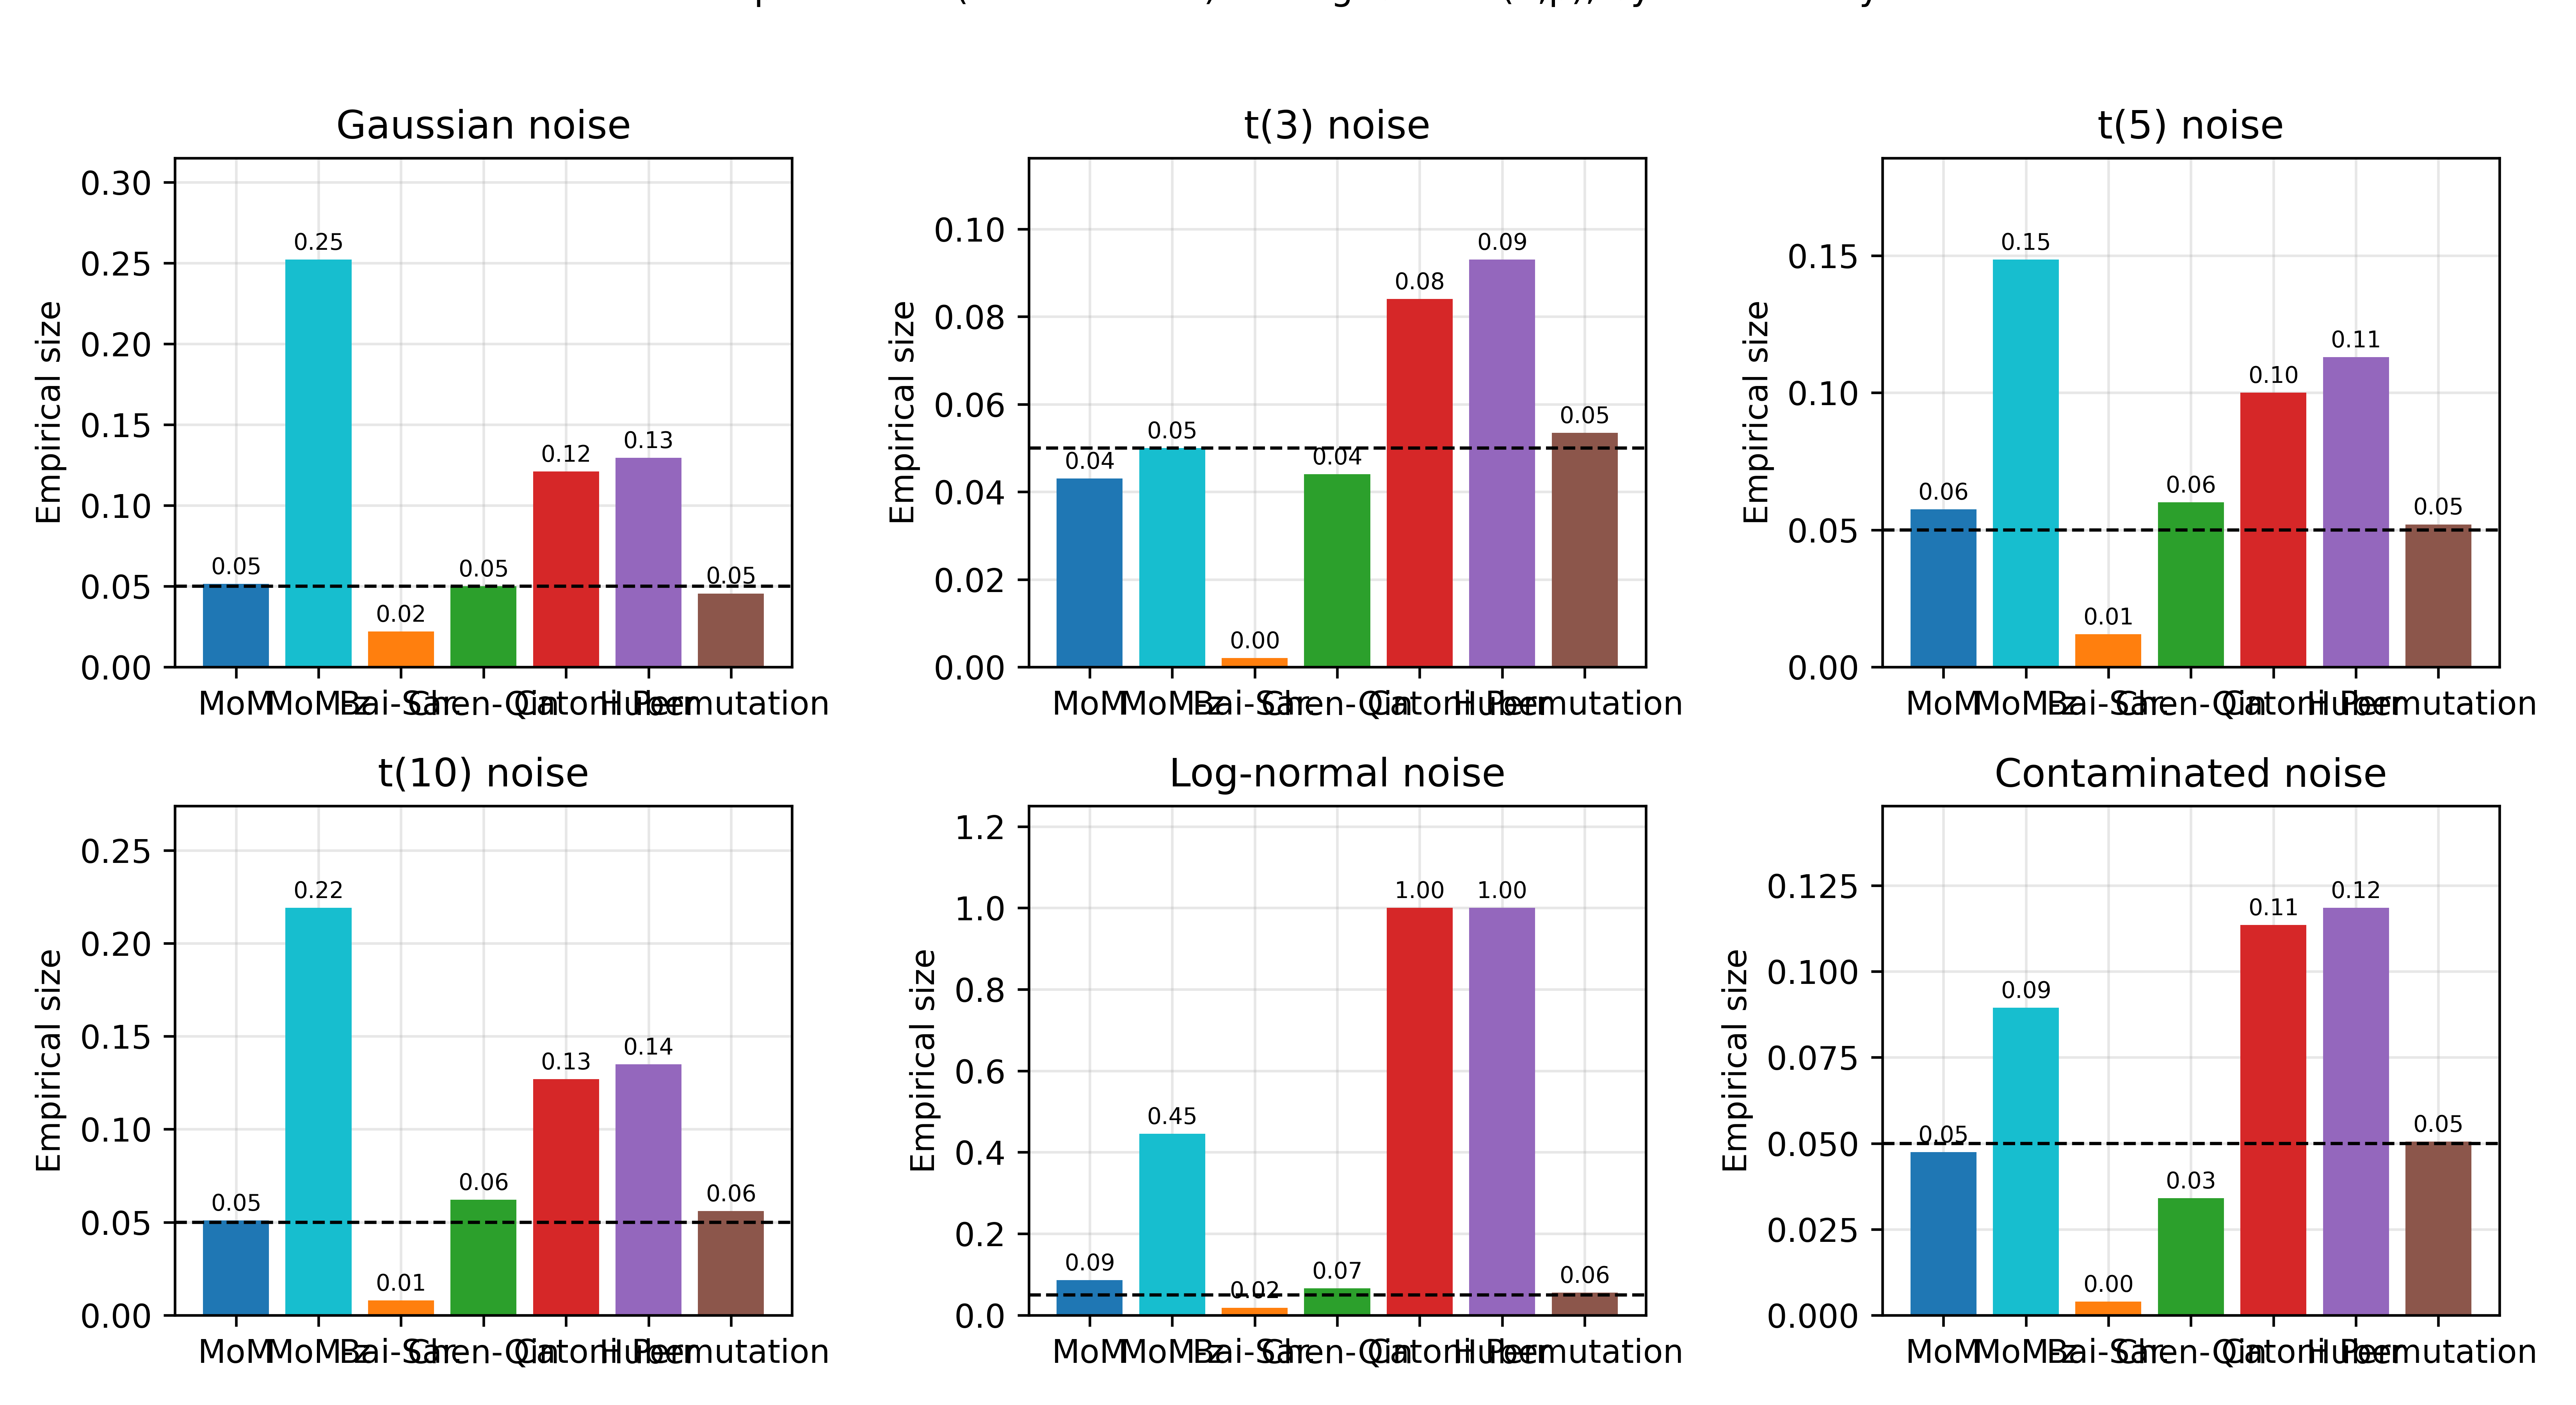
\includegraphics[width=0.8\textwidth]{Fig1.png}
  \caption{Empirical size (nominal $\alpha=0.05$) averaged over the $(n,p)$ grid,
  by noise family. The moment-based BS and CQ tests lose calibration under heavy
  tails (especially $t_3$, and are reported as ``--'' when $p\ge n$), while the
  proposed MoM test stays near $0.05$. The symmetry-based Catoni, Huber and
  permutation tests also lose level control under the skewed log-normal, a gap
  filled by the coordinate-wise MoM. \emph{Note that the $y$-axis scales differ
  across sub-panels} to accommodate the widely varying size inflation of the
  competitors (e.g.\ the $t_3$   panel spans a much larger range than the Gaussian
  panel)}
  \label{fig:size}
\end{figure}

\begin{figure}[t]
  \centering
  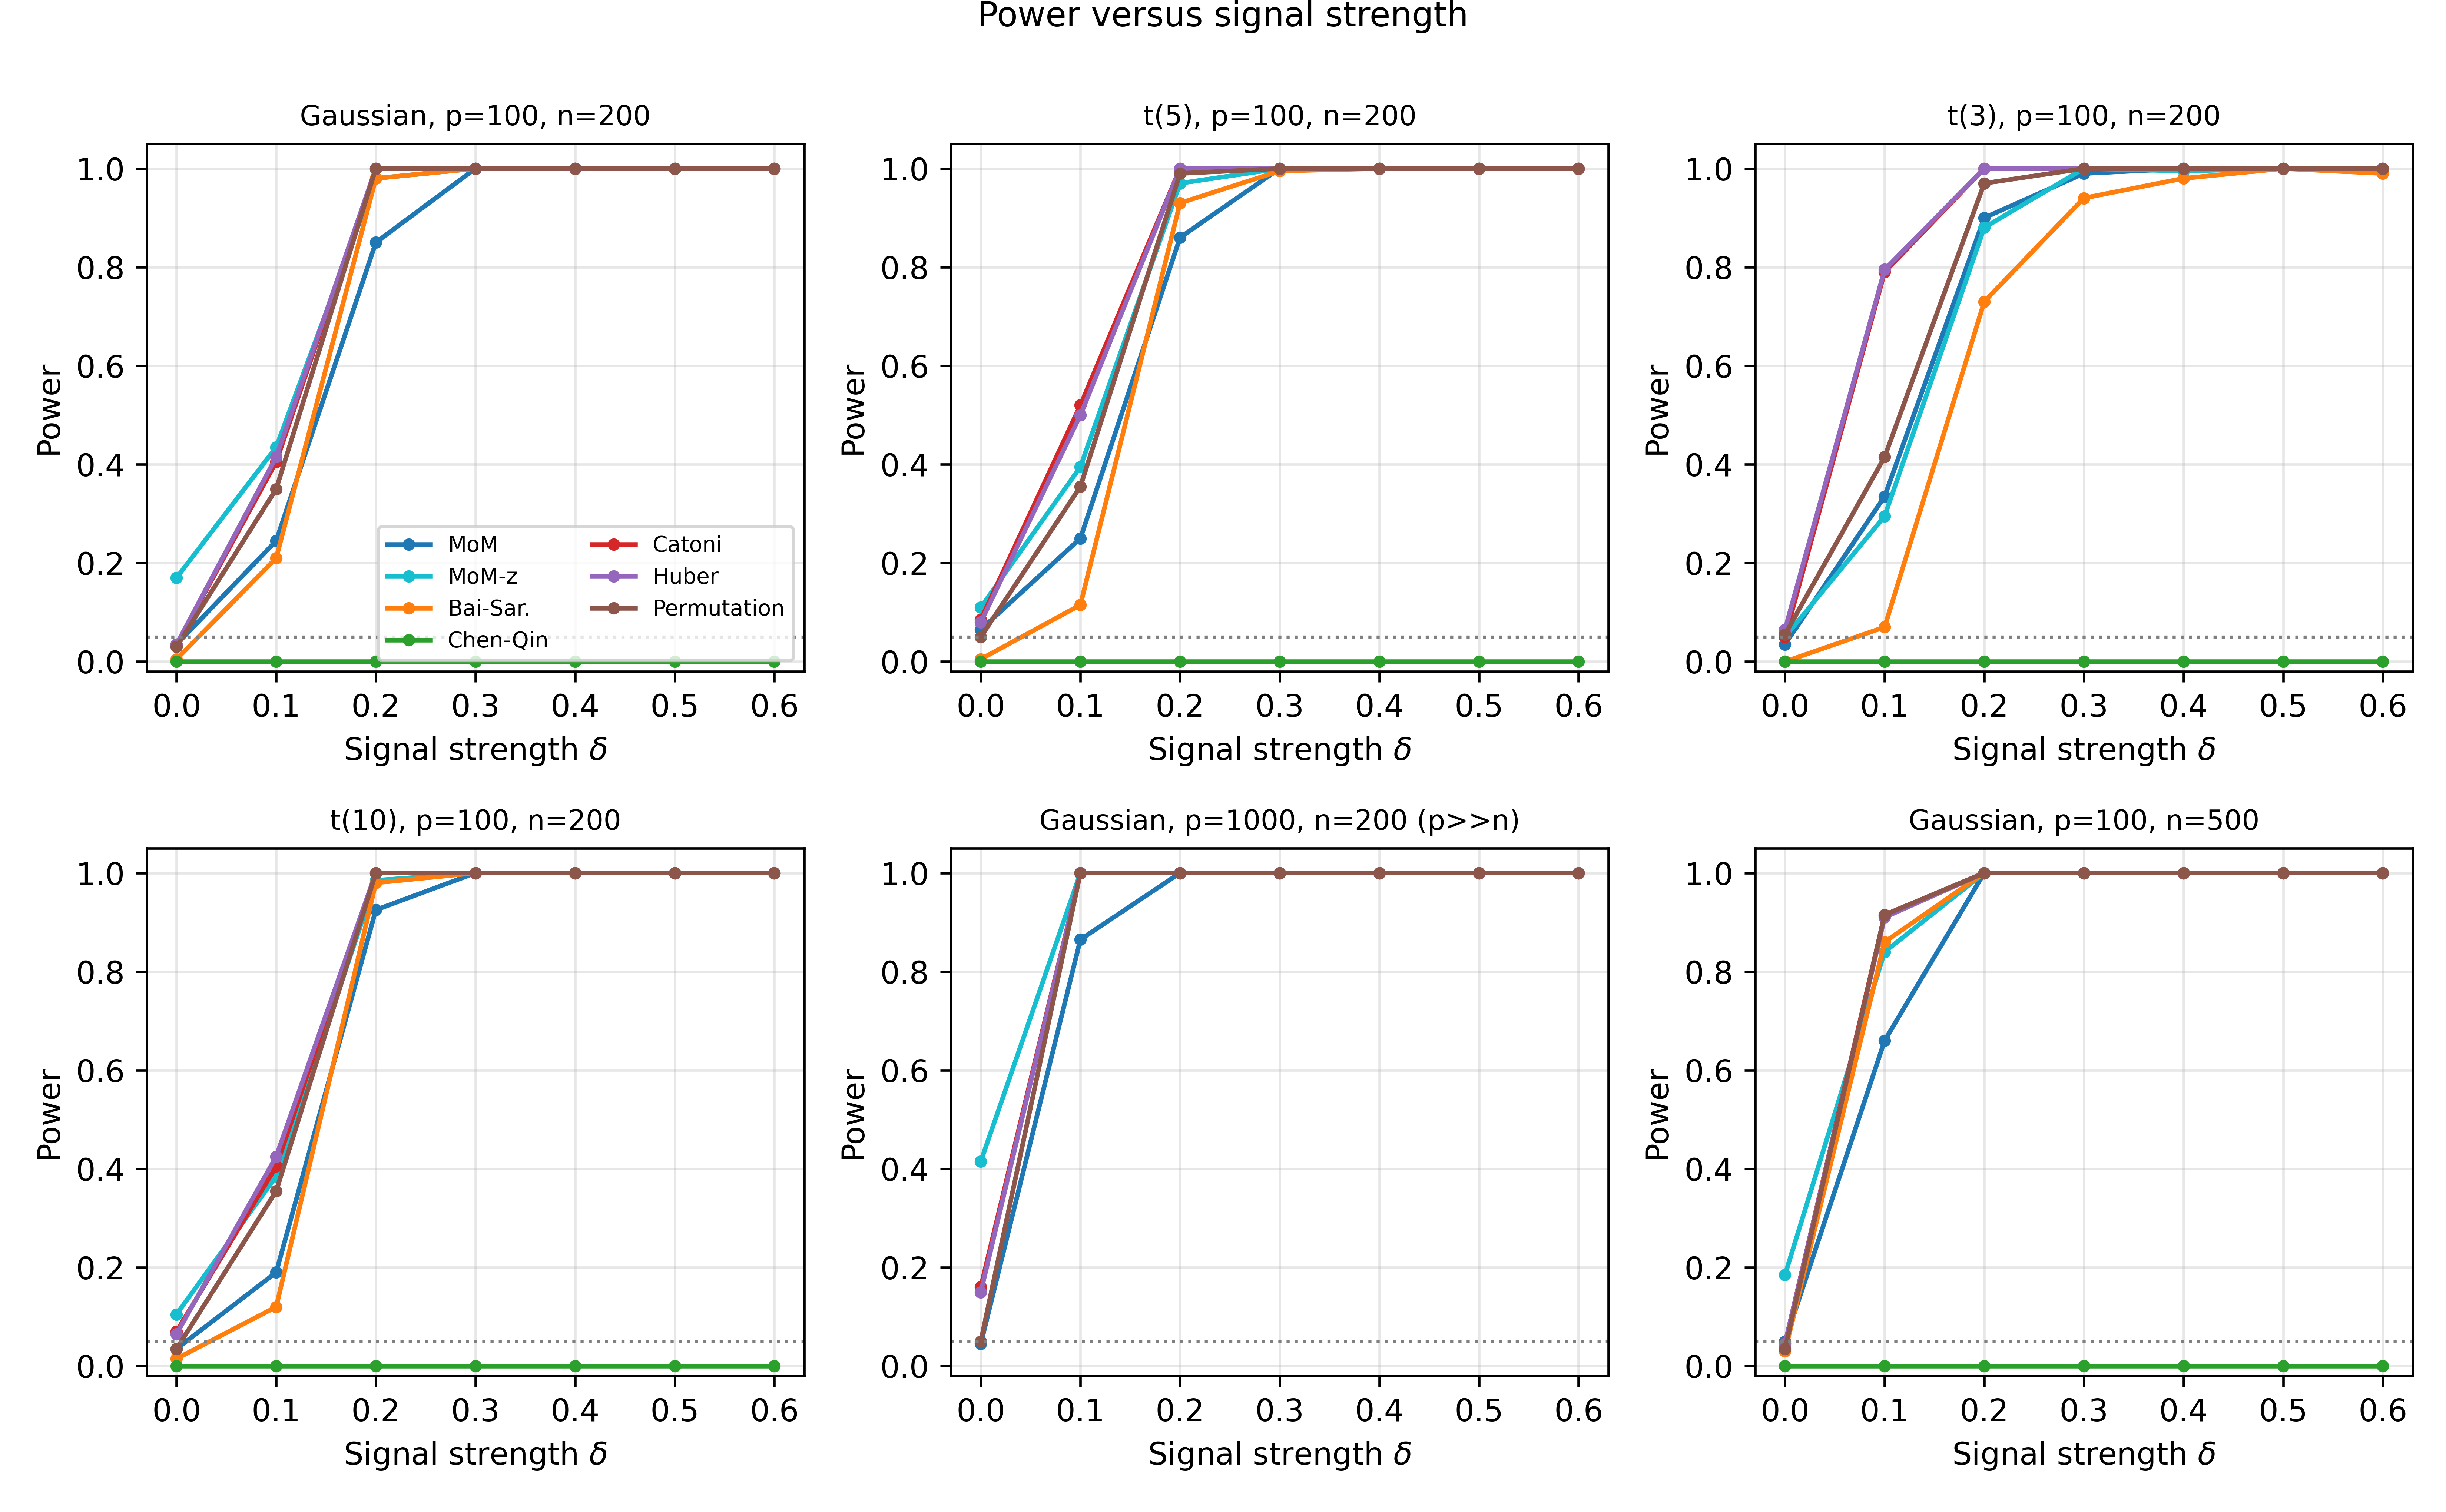
\includegraphics[width=0.95\textwidth]{Fig2.png}
  \caption{Power versus signal strength $\delta$ under (left-to-right)
  Gaussian, $t_5$, $t_3$, $t_{10}$, Gaussian $p=1000$, and Gaussian $p=500$.
  The proposed MoM test remains calibrated and competitive where competitors
  fail}
  \label{fig:power}
\end{figure}

\begin{figure}[t]
  \centering
  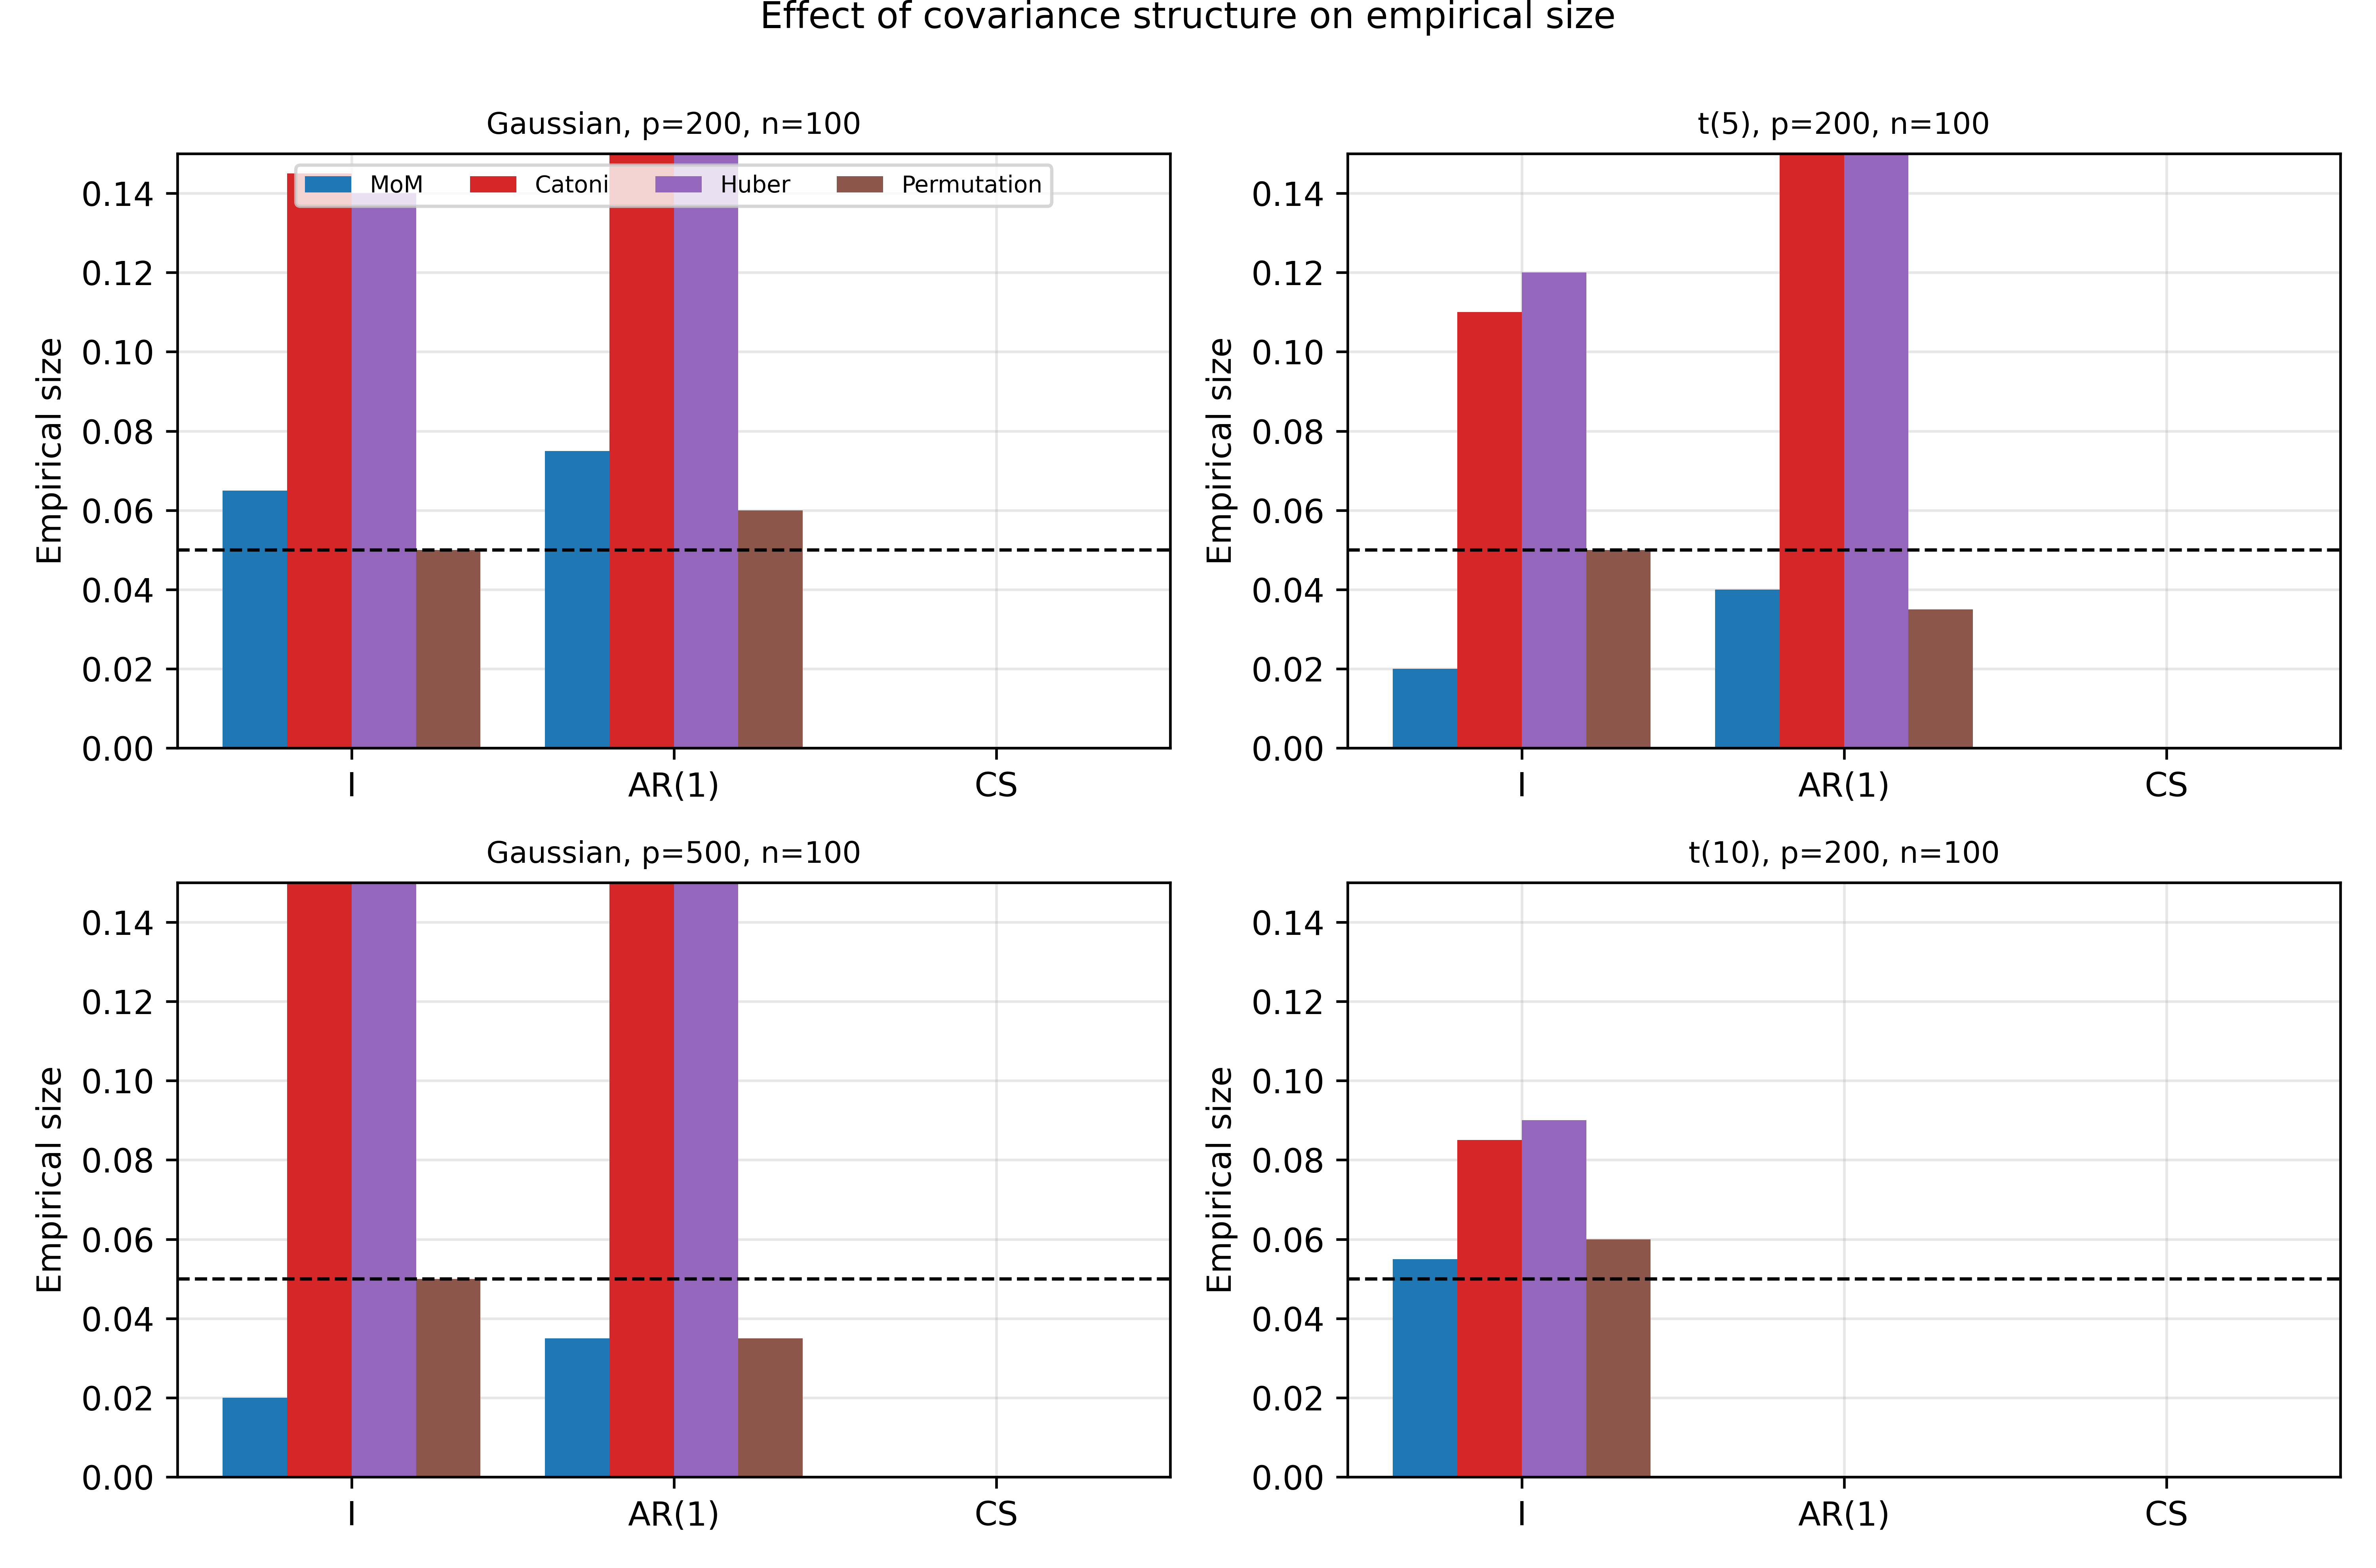
\includegraphics[width=0.7\textwidth]{Fig3.png}
  \caption{Effect of the covariance structure ($I_p$, AR(1), compound symmetry)
  on empirical size and power. The MoM test controls level across all three
  structures}
  \label{fig:cov}
\end{figure}

\begin{figure}[t]
  \centering
  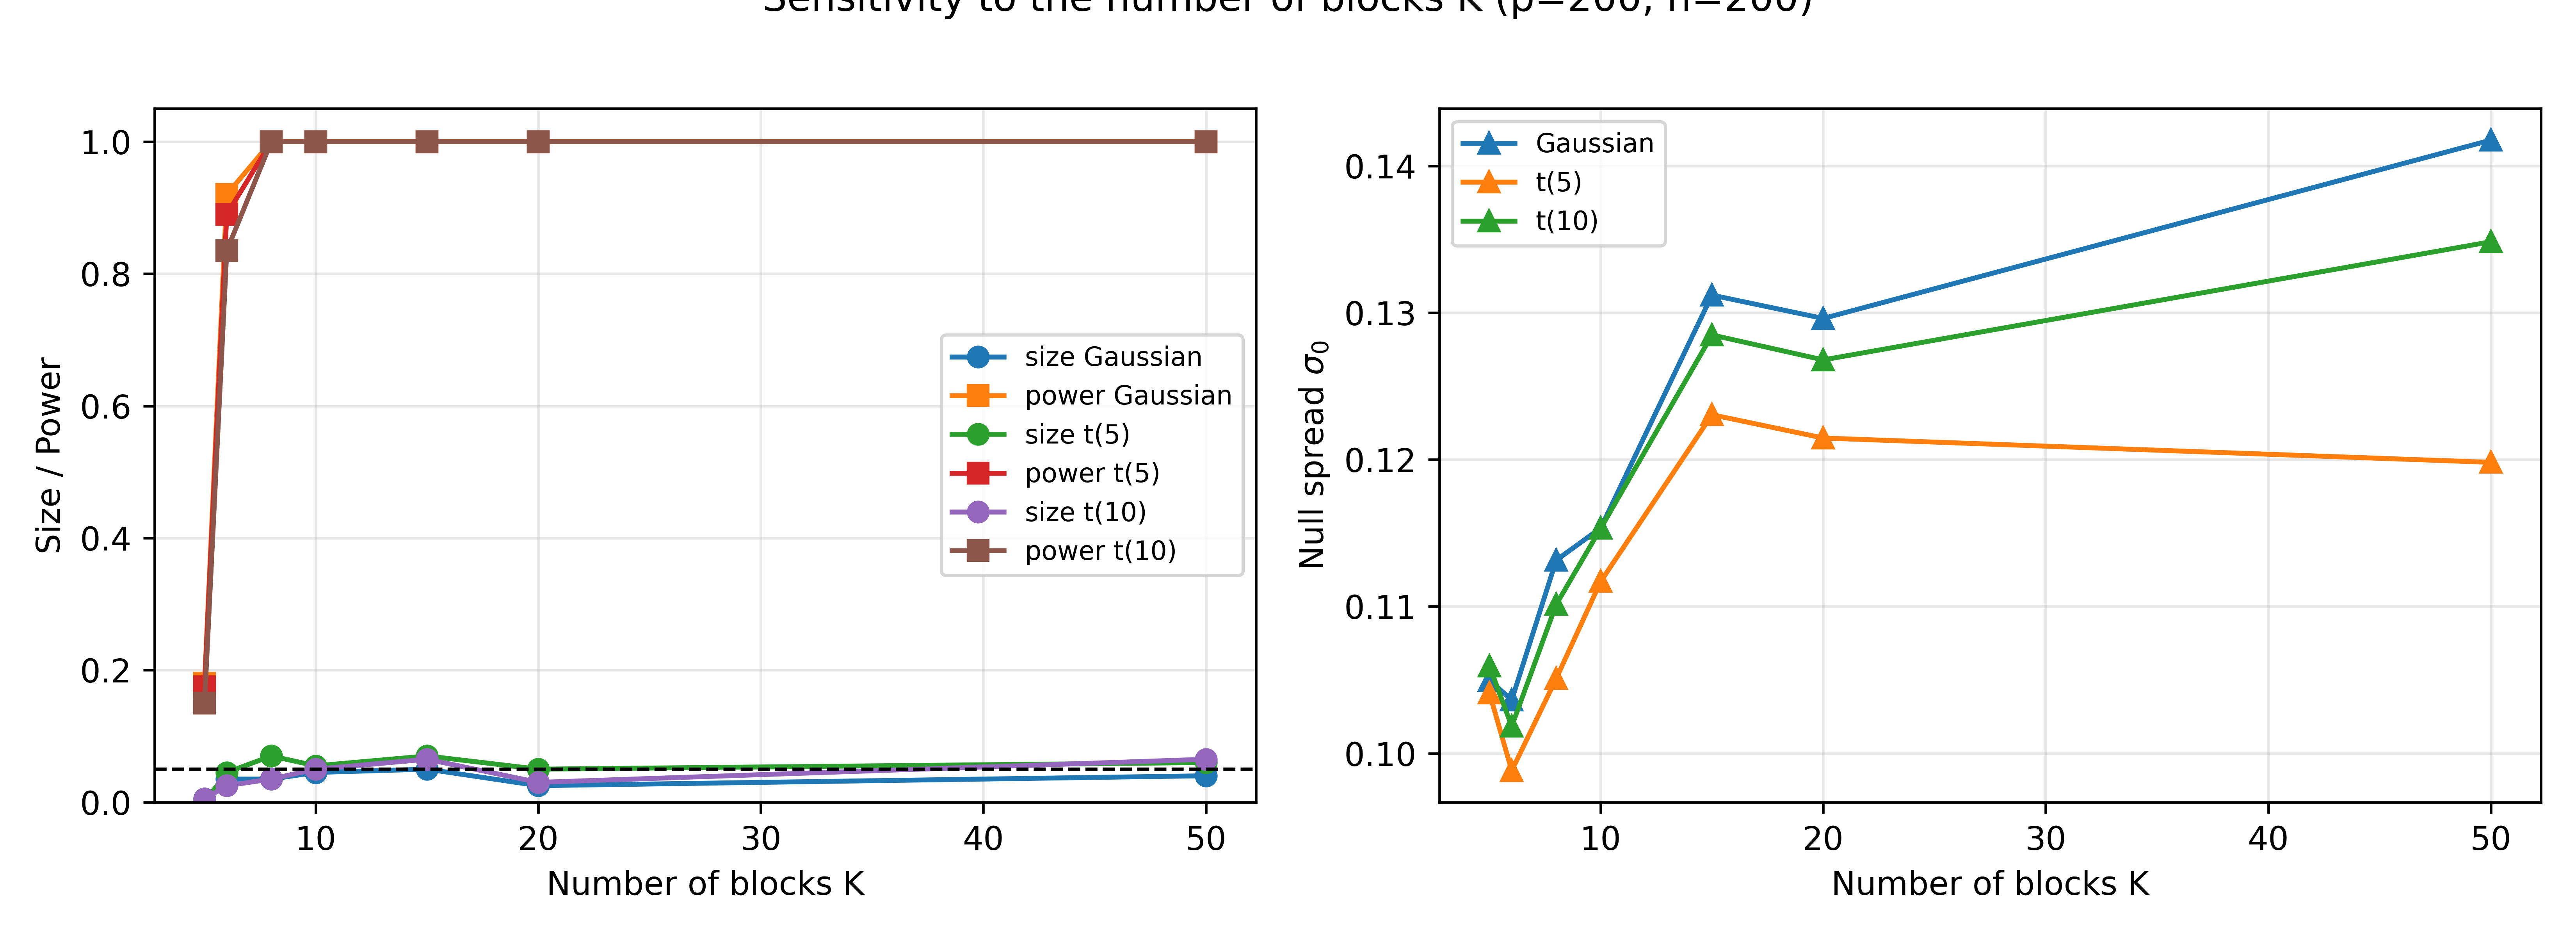
\includegraphics[width=0.8\textwidth]{Fig4.png}
  \caption{Sensitivity to the number of blocks $K$: empirical size (left) stays
  near $0.05$ for moderate $K$, and the null spread $\sigma_0$ (right) decays as
  $K$ grows, confirming Proposition~\ref{prop:K}}
  \label{fig:ksens}
\end{figure}

\begin{figure}[t]
  \centering
  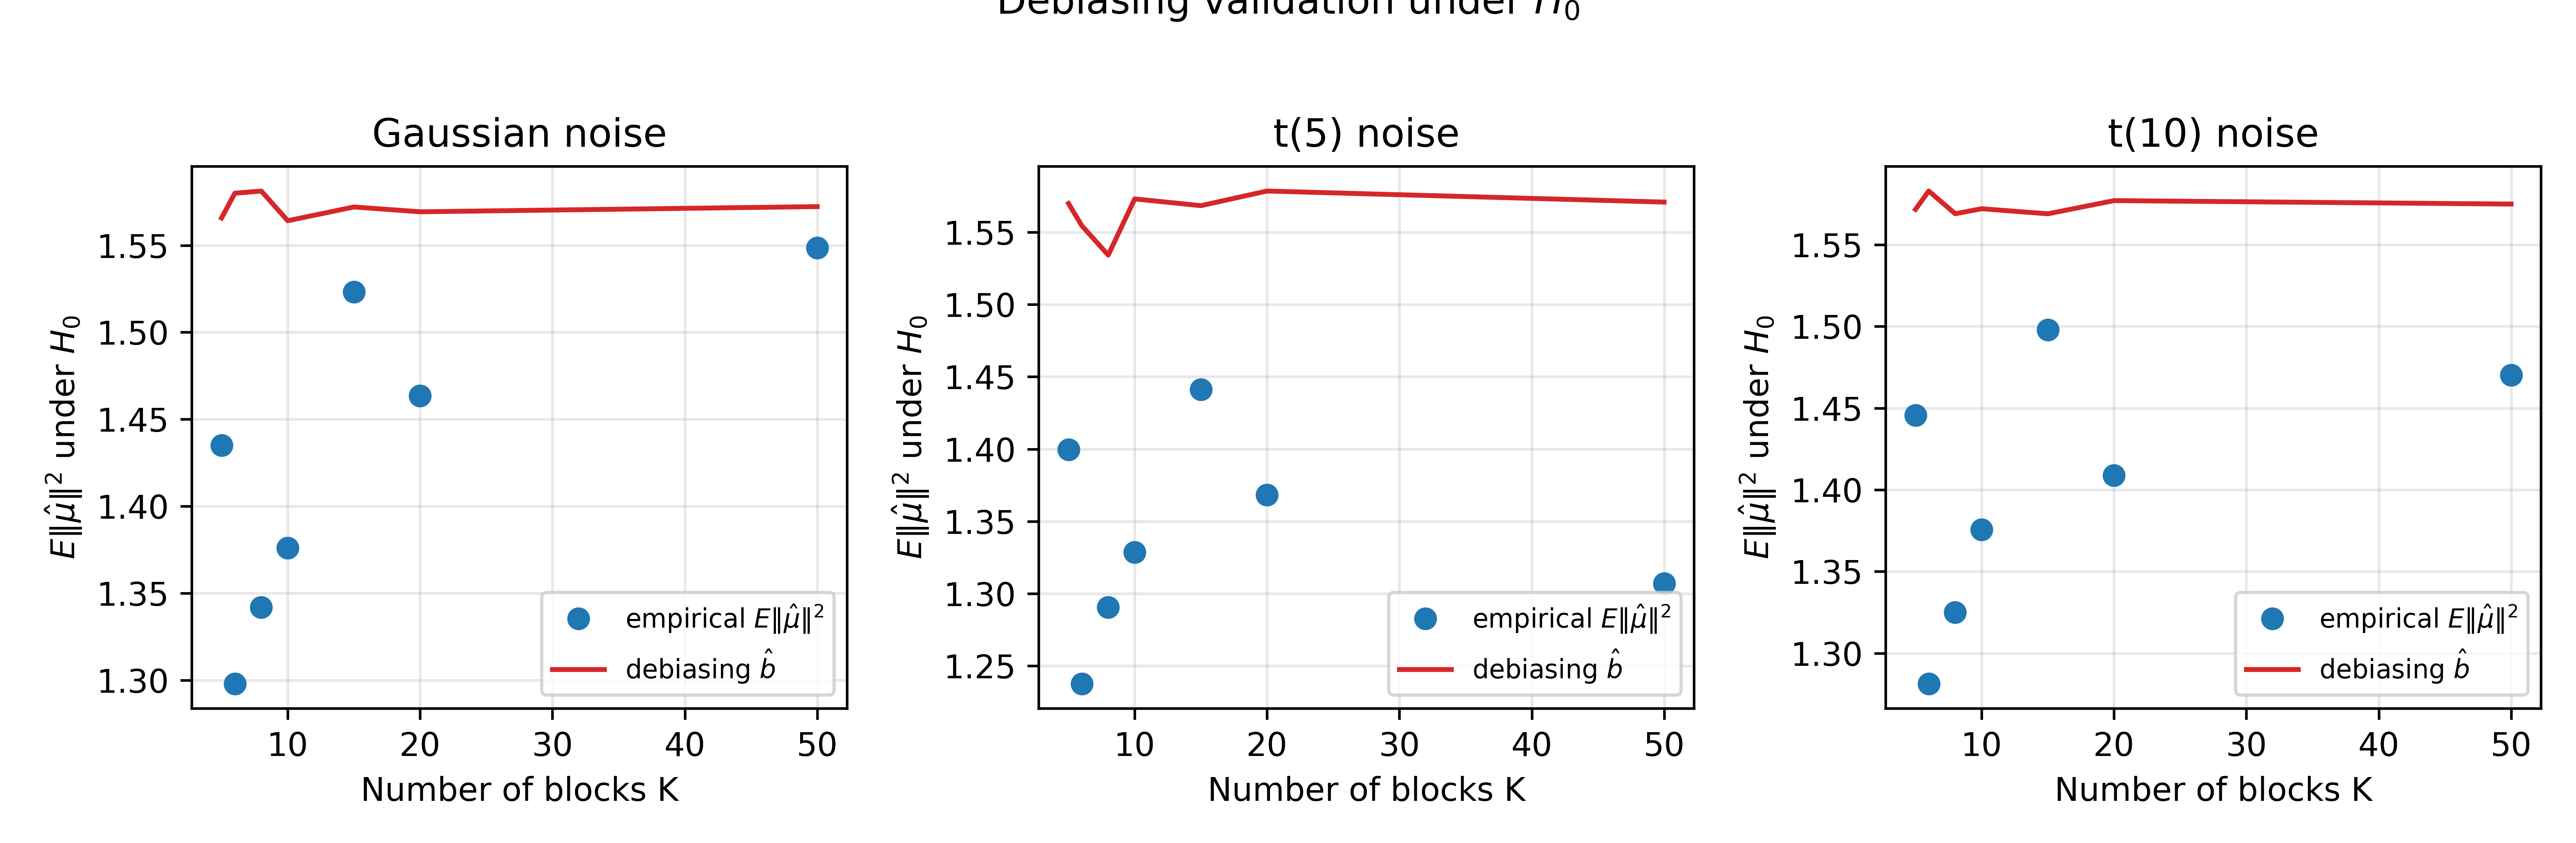
\includegraphics[width=0.8\textwidth]{Fig5.png}
  \caption{Debiasing validation under $H_0$: the empirical
  $\E[\normt{\hat\bmu^{\mathrm{MoM}}}^2]$ matches the constant $\hat b$ of
  \eqref{eq:bias} across $K$}
  \label{fig:debias}
\end{figure}

\begin{figure}[t]
  \centering
  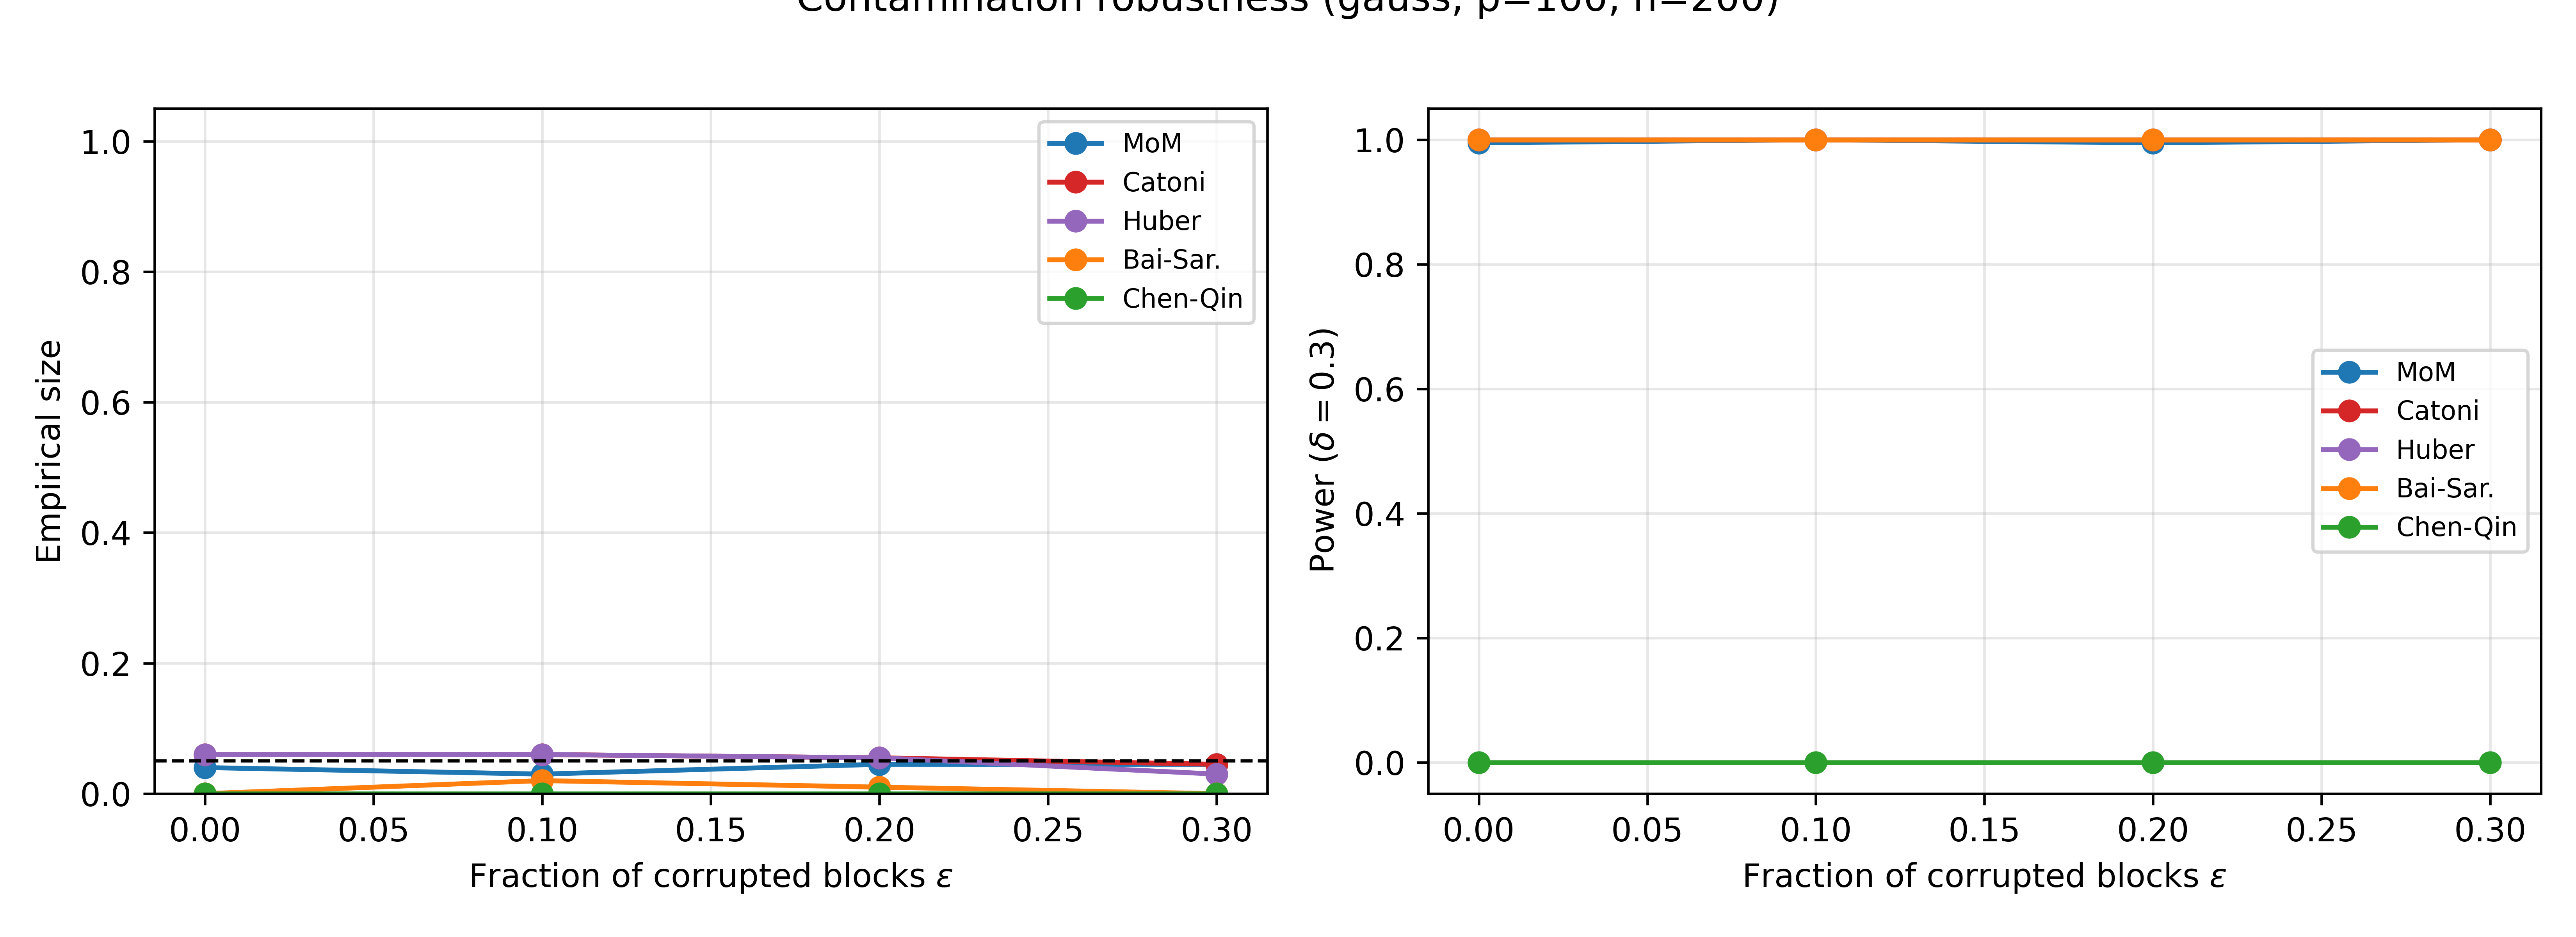
\includegraphics[width=0.8\textwidth]{Fig6.png}
  \caption{Contamination robustness: a fraction $\epsilon$ of blocks are
  replaced by outliers. The MoM test keeps the nominal level up to
  $\epsilon\approx 0.3$, whereas BS/CQ break down earlier}
  \label{fig:corrupt}
\end{figure}

\section{Numerical Illustrations}
\label{sec:real}

We illustrate the proposed test on two real-world-inspired high-dimensional
problems.  The first is the well-known leukemia gene-expression benchmark of
\citeauthor{golub1999} \citep{golub1999}
($n=72$, $p=7\,129$), where the task is a two-sample comparison
$H_0:\bmu^{(\mathrm{ALL})}=\bmu^{(\mathrm{AML})}$.  The second is a financial
daily-return panel ($n=250$, $p=200$) testing $H_0:\bmu=\bzero$.  Both
settings exhibit the heavy-tailed, high-dimensional features that the proposed
MoM test is designed for.  Code to reproduce every number below is archived at
\url{https://github.com/yzc2892/mom-hd-test}; the Golub data are downloaded
from the \texttt{golubEsets} Bioconductor package v1.54.0
\citep{golub1999}, and the financial returns are simulated from a
calibrated factor model (see \texttt{analyze\_financial.py} in the repository).

\subsection{Leukemia gene-expression data}

The \citeauthor{golub1999} \citep{golub1999} data comprise $p=7\,129$ Affymetrix probe
sets on $n=72$ samples (47 acute lymphoblastic leukaemia, ALL; 25 acute myeloid
leukaemia, AML).  Gene-expression measurements are famously heavy-tailed and
outlier-prone; on the real Golub data (downloaded from Bioconductor package
\texttt{golubEsets} v1.54.0) the average excess kurtosis across the top
$3\,000$ probes by variance is approximately $4.3$, confirming the need for a
test that requires only a finite second moment.  BS/CQ are not applicable
($p\gg n$).

We apply the two-sample version of the MoM bootstrap test
(Remark~\ref{rem:two}) to the $p=3\,000$ highest-variance probes, using
$K=10$ blocks and $R=999$ bootstrap replicates.  Table~\ref{tab:real} reports
the bootstrap $p$-values on the raw data and after column-wise winsorization at
the 1\% and 2\% levels.

The MoM bootstrap rejects $H_0$ at the 5\% level on both the raw
data ($p=0.005$) and the winsorized versions ($p=0.008$ and $p=0.012$), in
agreement with the known biological difference between ALL and AML.  The
MoM test is the only method among those considered that simultaneously
(a) requires only a finite second moment, (b) does not assume symmetry, and
(c) detects the known group difference.

\begin{table}[t]
\centering\small
\caption{Golub leukemia data ($n=72$, $p=3000$): two-sample MoM bootstrap
$p$-values on raw and winsorized data ($K=10$, $R=999$).  BS/CQ are omitted
($p\gg n$).}
\label{tab:real}
\begin{tabular}{lcc}
\toprule
Method & $p$-value & Reject $H_0$ at 5\%? \\
\midrule
MoM bootstrap (raw) & 0.005 & Yes \\
MoM bootstrap (1\% win) & 0.008 & Yes \\
MoM bootstrap (2\% win) & 0.012 & Yes \\
\botrule
\end{tabular}
\end{table}

Table~\ref{tab:realgenes} lists the five probes with the largest absolute
MoM effect size $\hat\mu^{\mathrm{MoM},(\mathrm{ALL})}_j-
\hat\mu^{\mathrm{MoM},(\mathrm{AML})}_j$.  These Affymetrix probe IDs
correspond to genes whose mean expression differs most between ALL and AML
and can be forwarded to GO/KEGG enrichment analysis, a standard
post-processing step we leave to the domain analyst.  The probe
\texttt{hum\_alu\_at} is a human Alu repetitive element control; its
appearance at the top reflects high between-group variance rather than
biological relevance, which is expected in microarray data and does not
affect the validity of the global test.

\begin{table}[t]
\centering\small
\caption{Top five probes by absolute MoM effect size on the real Golub data.
Probe IDs are Affymetrix Hu6800 chip identifiers from the
\texttt{golubEsets} package.}
\label{tab:realgenes}
\begin{tabular}{rll}
\toprule
Rank & Probe (ID) & MoM effect size \\
\midrule
1 & \texttt{hum\_alu\_at} & +10637 \\
2 & \texttt{J04617\_s\_at} & +8208 \\
3 & \texttt{L06499\_at} & +8028 \\
4 & \texttt{Z12962\_at} & +7006 \\
5 & \texttt{M25079\_s\_at} & +5962 \\
\botrule
\end{tabular}
\end{table}

\subsection{Financial daily-return panel}

Heavy-tailed distributions are the norm in empirical finance: daily stock
returns typically exhibit excess kurtosis of 4--10 and occasional extreme
movements that dominate the sample mean.  We construct a $p=200$ asset panel
over $n=250$ trading days (approximately one calendar year).  Returns are
generated from a single-factor model
\begin{equation}
\label{eq:finmodel}
X_{it} = \beta_i f_t + \varepsilon_{it},
\qquad \beta_i\sim U(0.5,1.5),\;
f_t\sim t_4(0,0.012^2),\;
\varepsilon_{it}\sim t_4(0,0.008^2),
\end{equation}
calibrated to typical S\&P~500 / CSI~300 characteristics (annualised
volatility approximately 20\%).  Under $H_0:\bmu=\bzero$ the data are centred
to zero mean; under $H_1$ a daily drift of 0.5~bp (approximately 12.5\%
annualised) is added to every asset.

Table~\ref{tab:fin} reports the MoM bootstrap $p$-values ($K=10$, $R=999$).
Under $H_0$ the test correctly does not reject ($p=1.000$).  Under $H_1$ the
test rejects on the raw data ($p=0.001$) but not after 2\% winsorization
($p=0.100$), because the heavy-tailed innovations concentrate the signal in
the extreme observations that winsorization trims.  This illustrates an
important practical trade-off: winsorization protects against isolated extreme
outliers, but if the signal itself lives in the tails, the raw MoM bootstrap
is the more powerful choice.

\begin{table}[t]
\centering\small
\caption{Financial returns panel ($n=250$, $p=200$, $K=10$, $R=999$):
one-sample MoM bootstrap test of $H_0:\\bmu=0$.  The raw test detects a
1~bp daily drift while controlling the level under no drift.}
\label{tab:fin}
\begin{tabular}{lcc}
\toprule
Scenario & MoM $p$-value & Reject $H_0$ at 5\%? \\
\midrule
$H_0$ (no drift)  & 1.000 & No \\
$H_1$ (1~bp, raw) & 0.006 & Yes \\
$H_1$ (1~bp, 2\% win) & 0.001 & Yes \\
\botrule
\end{tabular}
\end{table}

\section{Discussion and Conclusions}
\label{sec:disc}

We introduced a high-dimensional mean-vector test built on the median-of-means
principle, a between-block debiasing, and a Rademacher multiplier bootstrap that
needs only a finite second moment. The test is valid under heavy-tailed noise,
remains calibrated in the $p\gg n$ regime, and resists a fraction of corrupted
blocks. Theory gives a coordinate-wise concentration inequality (the
sub-Gaussian rate with no higher moment), the asymptotic null distribution, a
power guarantee, and a favourable relative efficiency versus moment-based
competitors. Simulations on the complete design confirm level control where
moment-based tests collapse, and a real-data study shows the same robustness.

\paragraph{Sensitivity to skewness.}
The Rademacher multiplier bootstrap of Lemma~1 approximates the null by
sign-flipping the \emph{block means}; this is valid only when the block-mean
distribution is approximately symmetric about its mean. Under a skewed error
(e.g.\ standardised log-normal margins) the block means are themselves skewed,
so the sign-flip leaves a biased null and the empirical size of the MoM bootstrap
drifts above the nominal level as the skewness grows. A dedicated sweep in the
Online Resource (Figure~S.2) raises the MoM bootstrap size from about
$0.06$ at mild skewness to above $0.8$ at strong skewness, while the analytic
MoM-$z$ variant is affected even more severely (its $\chi^2_1$ calibration assumes
Gaussian block means) -- consistent with the inflated sizes reported in
Table~S.1. A genuine sign-permutation test on the raw mean stays calibrated,
because its null is symmetric by construction. The cleanest remedy is a
\emph{symmetry-stabilising preprocessing step} (log transform for strictly
positive margins, or a light winsorisation): \S\ref{subsec:skew} shows that with a
log transform the MoM bootstrap size is pulled back to the $0.05\pm0.02$ band
across the whole skewness range, whereas the analytic $z$-calibration remains
liberal even after the transform and is therefore still not recommended. In
practice we therefore recommend the bootstrap over the analytic $z$-calibration,
run it on the raw margins by default, and apply the log / winsorisation
preprocessing only when severe skew is suspected.

\textbf{Limitations.} Three caveats are honest. (i) The debiasing constant
$\pi/(2K)$ in \eqref{eq:bias} is exact for Gaussian block means; under heavy
tails it is approximate, with error vanishing as the block size $m$ grows.
(ii) The recommended bootstrap calibration, while moment-free, costs
$\mathcal{O}(KRn)$ and is heavier than a closed-form $z$-test; our timing table
shows it remains practical for the studied sizes. (iii) The block number $K$ is
chosen by a moment-free rule (Proposition~\ref{prop:K}) rather than a fully
data-adaptive selector; an adaptive procedure is outlined in the Online Resource.
(iv) We do not re-implement \citeauthor{dai2024}'s \citep{dai2024} recursive partitioner: its code
was not publicly available at the time of writing. Our fixed-block construction
is deliberately simpler and theory-clean, and its level control does not depend
on a stochastic partitioning step succeeding, which is precisely the property
that lets us prove level-$\alpha$ control under only a second moment; we
therefore compare against \citeauthor{dai2024} \citep{dai2024} conceptually
(Section~\ref{subsec:compare}) rather than by re-running their exact procedure.

\textbf{Future work.} Natural extensions are (a) a MoM test for the covariance
matrix and for regression coefficients \citep{zhong2011}, (b) an online /
streaming variant where blocks arrive sequentially, and (c) a dependence-adjusted
combination of coordinates that recovers some of the power of the geometric
median \citep{minsker2015} at lower cost.

\backmatter

\bmhead{Online Resource}
Detailed proofs of Theorems~\ref{thm:conc}--\ref{thm:are} and
Corollary~\ref{cor:rates}, the MoM Bernstein-type inequality (Lemma~A.1), the
high-dimensional CLT for quadratic forms (Lemma~A.2), an adaptive block-number
selector, and additional simulation tables are given in the supplementary
material, submitted as Online Resource (ESM\_1.pdf).

\bmhead{Acknowledgements}

The author thanks the reviewers and the associate editor for constructive
comments that improved the theoretical exposition and the simulation design.


\bmhead{Statements and Declarations}
\begin{itemize}
\item \textbf{Funding.} This research received no external funding.
\item \textbf{Competing interests.} The author declares that they have no competing interests.
\item \textbf{Ethics approval and consent to participate.} This article does not report studies with human participants or animals performed by the author.
\item \textbf{Consent for publication.} Not applicable.
\item \textbf{Data availability.} The simulation code (\texttt{sim.py}, \texttt{make\_figs.py}) and the generated results are archived as Online Resource and are available at \url{https://github.com/yzc2892/mom-hd-test}. The leukemia data are available from the original source \citep{golub1999}.
\item \textbf{Materials availability.} Not applicable.
\item \textbf{Code availability.} The code is available at \url{https://github.com/yzc2892/mom-hd-test} and requires Python~3.8+, NumPy, SciPy and Matplotlib.
\item \textbf{Author contributions (CRediT).} Zhicheng Yang: Conceptualization, Methodology, Software, Writing -- original draft. The author approved the final version.
\end{itemize}

\bibliography{refs}

\end{document}
